\documentclass{../latex/analysis_report}

\usepackage{longtable}

\reporttitle{Exploratory Data Analysis: Subiculum Literature Dataset}
\reportauthor{Kyle Shannon}
\reportdate{December 2025}

\begin{document}

\maketitle

\section{Summary}

This EDA examines 59 years of subiculum research literature extracted from PubMed. The dataset contains 3,576 papers spanning from 1966 to 2025, with 15,603 unique authors publishing across 593 journals. The analysis reveals significant growth in subiculum research, particularly after 2010, with strong representation of neuroimaging, Alzheimer's disease, and neuroanatomy studies.

\vspace{8pt}
\noindent\textbf{Key Findings:}
\vspace{-2pt}
\begin{itemize}[noitemsep,topsep=0pt]
    \item Research has accelerated dramatically: 39\% of all papers published in the last decade
    \item The Journal of Neuroscience and Brain Research dominate the publication landscape
    \item 91\% of papers include MeSH term annotations enabling semantic analysis
    \item Citation enrichment achieved 80\% coverage through CrossRef/Semantic Scholar integration
    \item Neuroanatomy and Alzheimer's disease represent the largest research themes
\end{itemize}

\section{Dataset Overview}

\subsection{Coverage Statistics}

The dataset shows excellent metadata completeness, with nearly all papers including titles (100\%), abstracts (98.5\%), and DOIs (95.7\%). This high quality enables future text mining and semantic analysis.

\begin{table}[htbp]
\centering
\caption{Dataset coverage statistics}
\label{tab:coverage}
\begin{tabular}{lrr}
\toprule
\textbf{Metric} & \textbf{Value} & \textbf{Percentage} \\
\midrule
Total Papers & 3,576 & 100\% \\
Year Range & 1966 -- 2025 & 59 years \\
Papers with Abstracts & 3,521 & 98.5\% \\
Papers with DOI & 3,423 & 95.7\% \\
Papers with PMC ID & 1,419 & 39.7\% \\
Average Text Length & 1,621 chars & --- \\
\bottomrule
\end{tabular}
\end{table}

\begin{figure}[htbp]
\centering
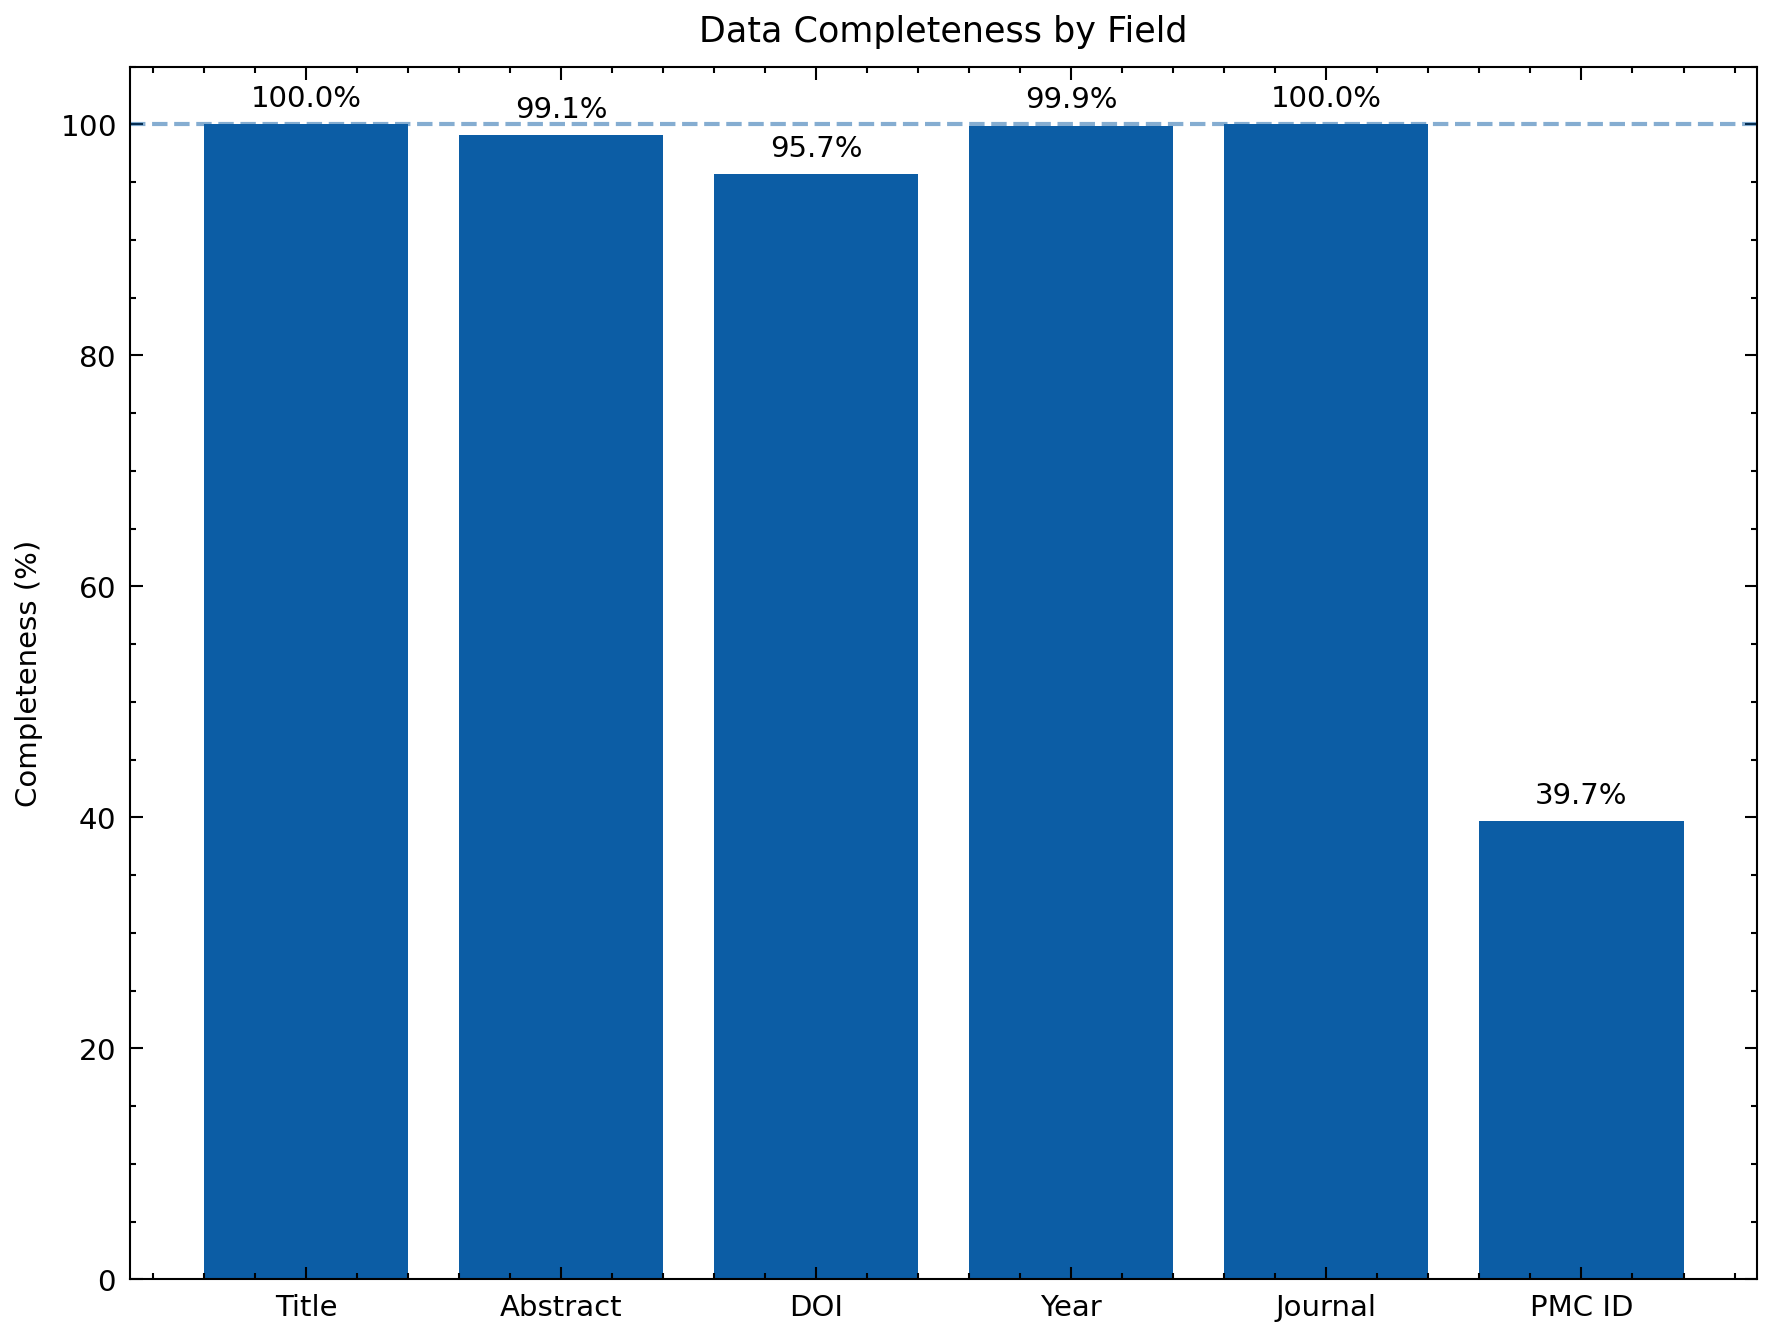
\includegraphics[width=0.8\textwidth]{imgs/general_eda_2025-12-06_data_completeness.png}
\caption{Data completeness by field showing high quality metadata across core bibliographic fields.}
\label{fig:completeness}
\end{figure}

\section{Temporal Trends}

\subsection{Publication Growth}

Subiculum research has grown substantially over six decades. The 2010s marked a peak in publication volume with 904 papers (25\% of the entire dataset). The slight decline in the 2020s reflects incomplete data for 2025-2029 and COVID-19 impacts.

\begin{table}[htbp]
\centering
\caption{Publication volume by decade}
\label{tab:decades}
\begin{tabular}{lrr}
\toprule
\textbf{Decade} & \textbf{Papers} & \textbf{Growth from Previous} \\
\midrule
1960s & 1 & --- \\
1970s & 55 & +5400\% \\
1980s & 358 & +551\% \\
1990s & 717 & +100\% \\
2000s & 667 & -7\% \\
2010s & 904 & +36\% \\
2020s & 870 & -4\% \\
\bottomrule
\end{tabular}
\end{table}

\begin{figure}[htbp]
\centering
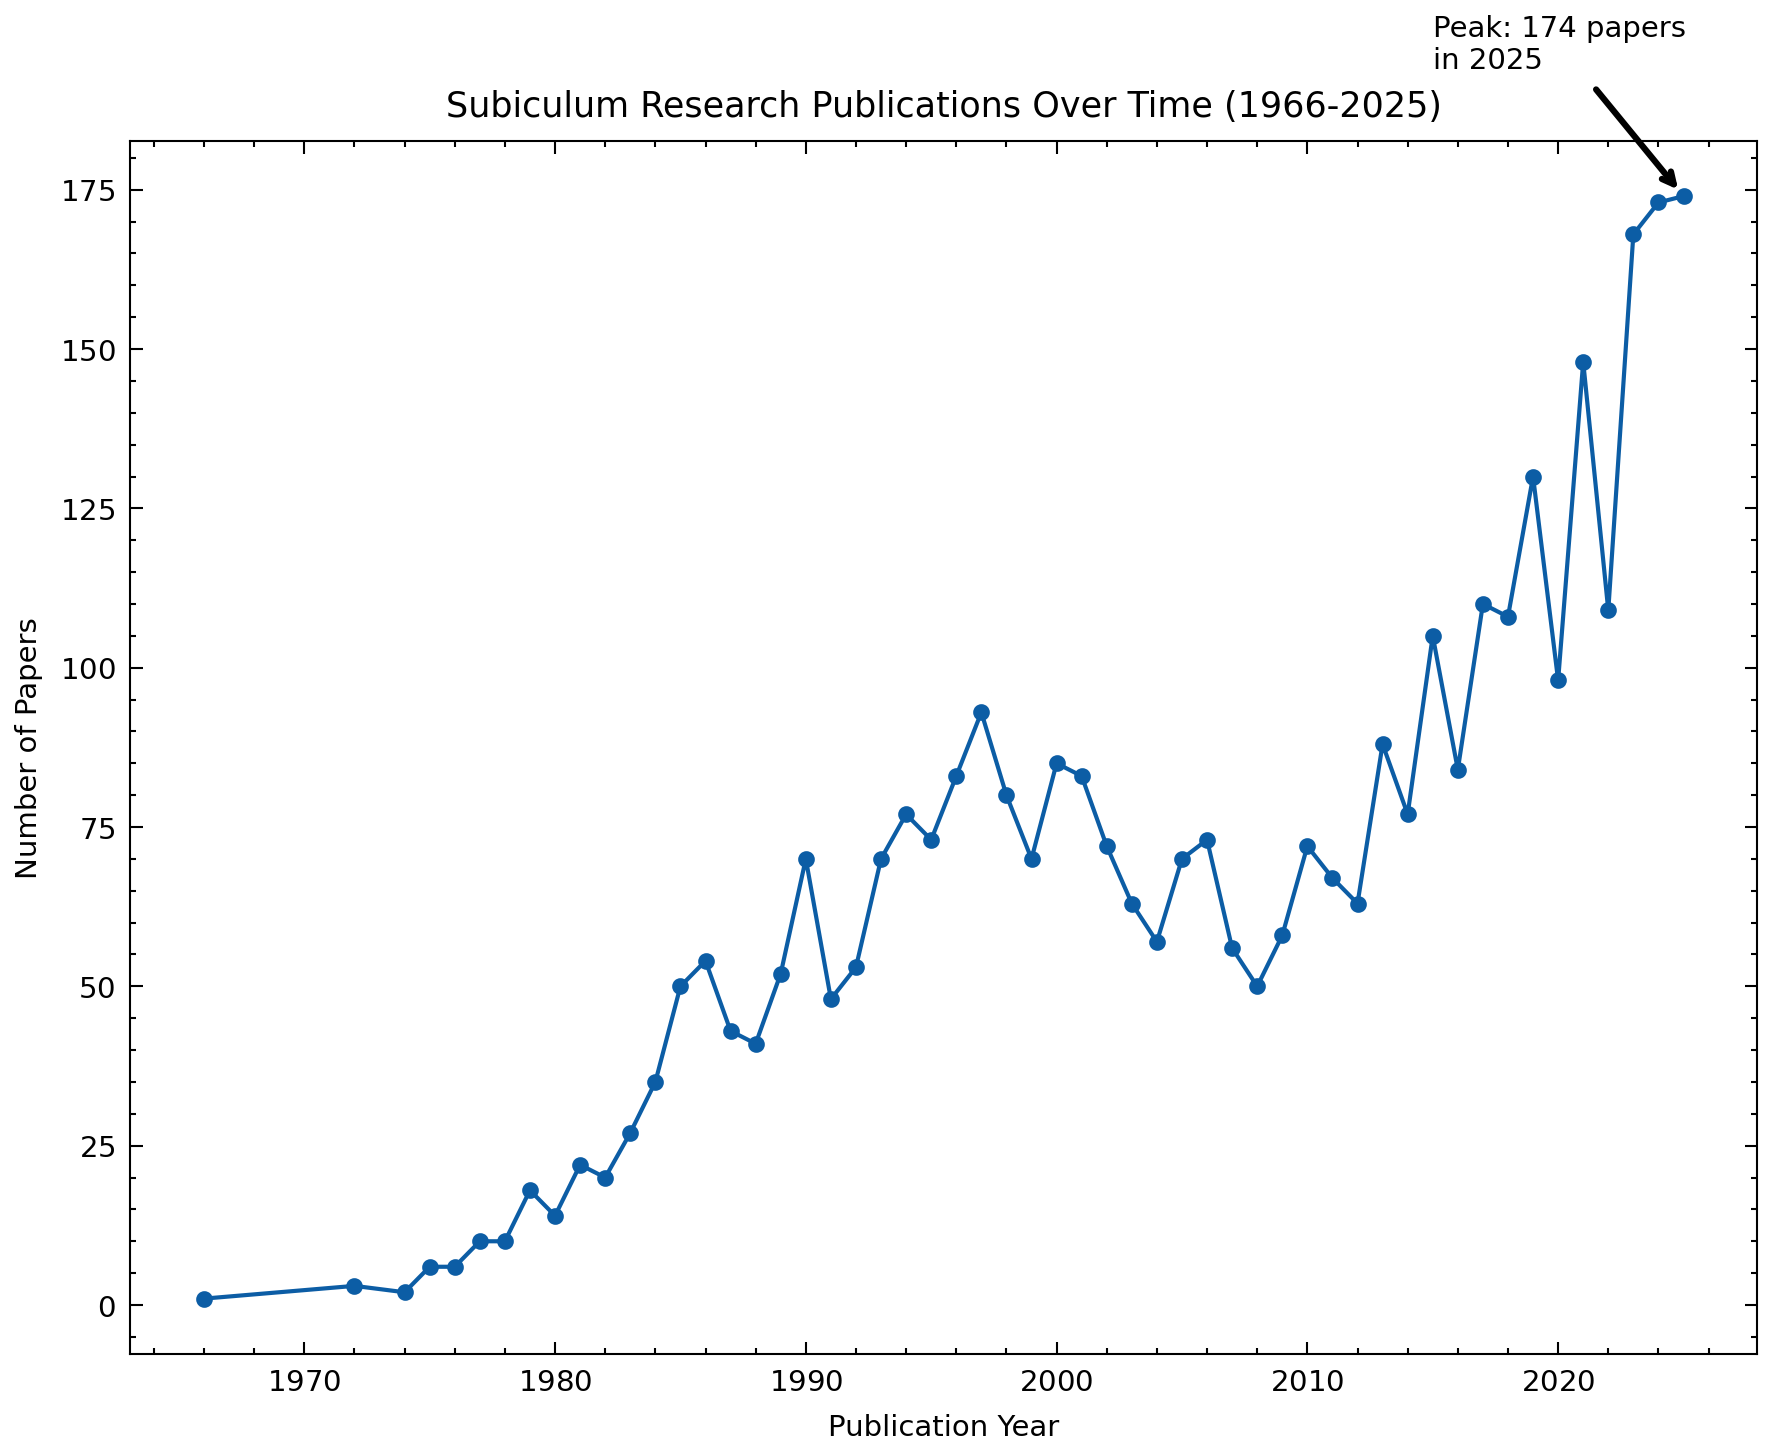
\includegraphics[width=\textwidth]{imgs/general_eda_2025-12-06_papers_by_year.png}
\caption{Annual publication counts showing sustained growth from 1966 to 2025, with peak years in 2020-2024.}
\label{fig:papers_year}
\end{figure}

\subsection{Recent Acceleration}

The last 10 years (2015-2025) account for 1,407 papers (39\% of total), with an average of 128 papers per year. The 5-year moving average shows sustained growth, peaking at approximately 150 papers per year in 2020-2024.

\begin{figure}[htbp]
\centering
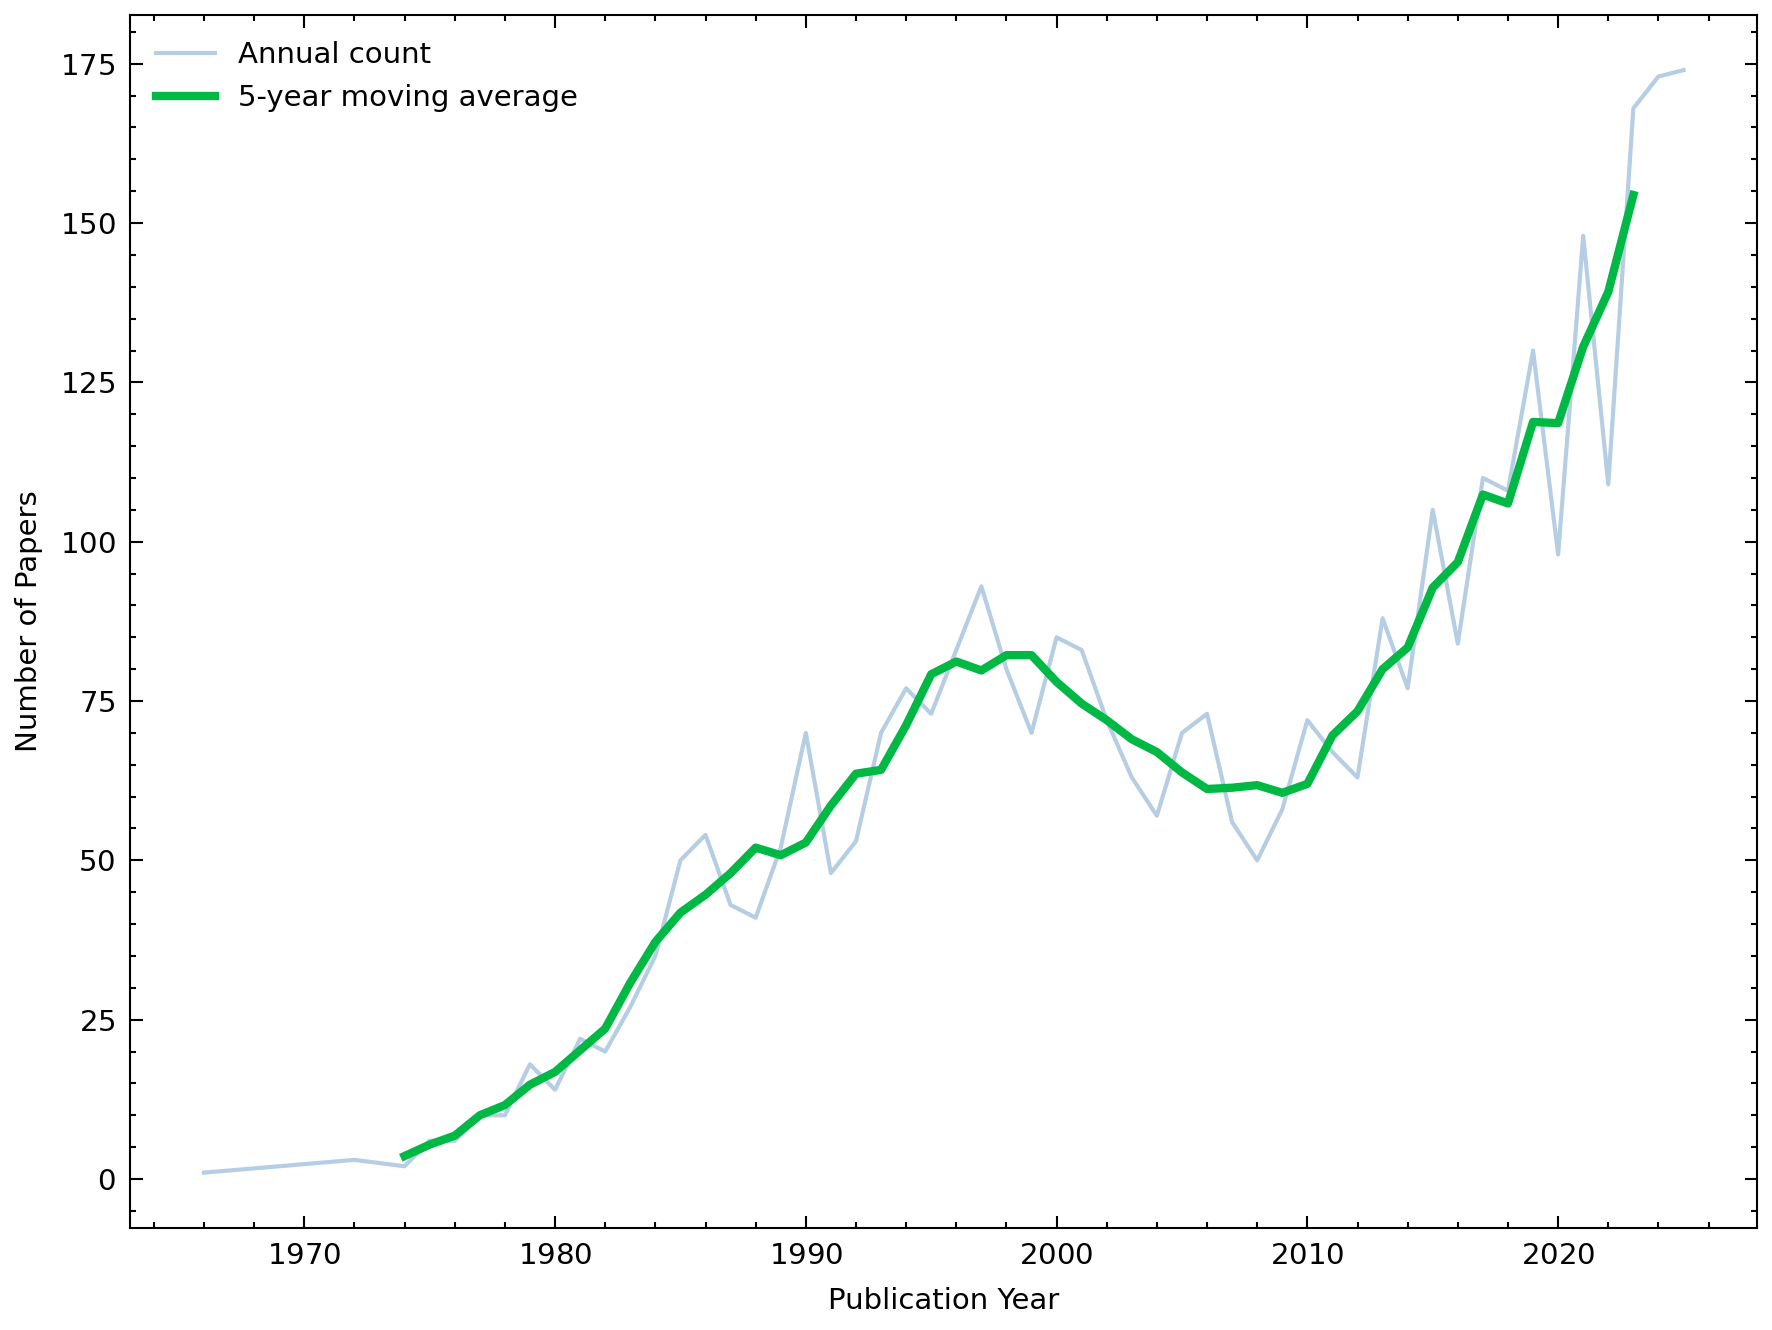
\includegraphics[width=\textwidth]{imgs/general_eda_2025-12-06_publication_acceleration.png}
\caption{Publication acceleration shown through 5-year moving average, revealing steady growth with recent peak.}
\label{fig:acceleration}
\end{figure}

\textbf{Key Observation:} The 2023-2025 period shows the highest sustained publication rate in subiculum research history (173-174 papers per year).

\section{Journal Distribution}

\subsection{Top Publishing Venues}

Subiculum research is published across 593 unique journals, with the top 10 accounting for 31.9\% of all papers.

\begin{table}[htbp]
\centering
\caption{Top 10 journals by paper count with PMC access rates}
\label{tab:journals}
\small
\begin{tabular}{rlrr}
\toprule
\textbf{Rank} & \textbf{Journal} & \textbf{Papers} & \textbf{PMC Access} \\
\midrule
1 & Brain Research & 218 & 4.1\% \\
2 & Journal of Comparative Neurology & 212 & 10.4\% \\
3 & Neuroscience & 166 & 7.2\% \\
4 & Hippocampus & 128 & 28.9\% \\
5 & Journal of Neuroscience & 122 & 100\% \\
6 & European Journal of Neuroscience & 65 & 16.9\% \\
7 & Neuroscience Letters & 62 & 1.6\% \\
8 & Acta Neuropathologica & 57 & 15.8\% \\
9 & Behavioural Brain Research & 57 & 12.3\% \\
10 & NeuroImage & 54 & 44.4\% \\
\bottomrule
\end{tabular}
\end{table}

\begin{figure}[htbp]
\centering
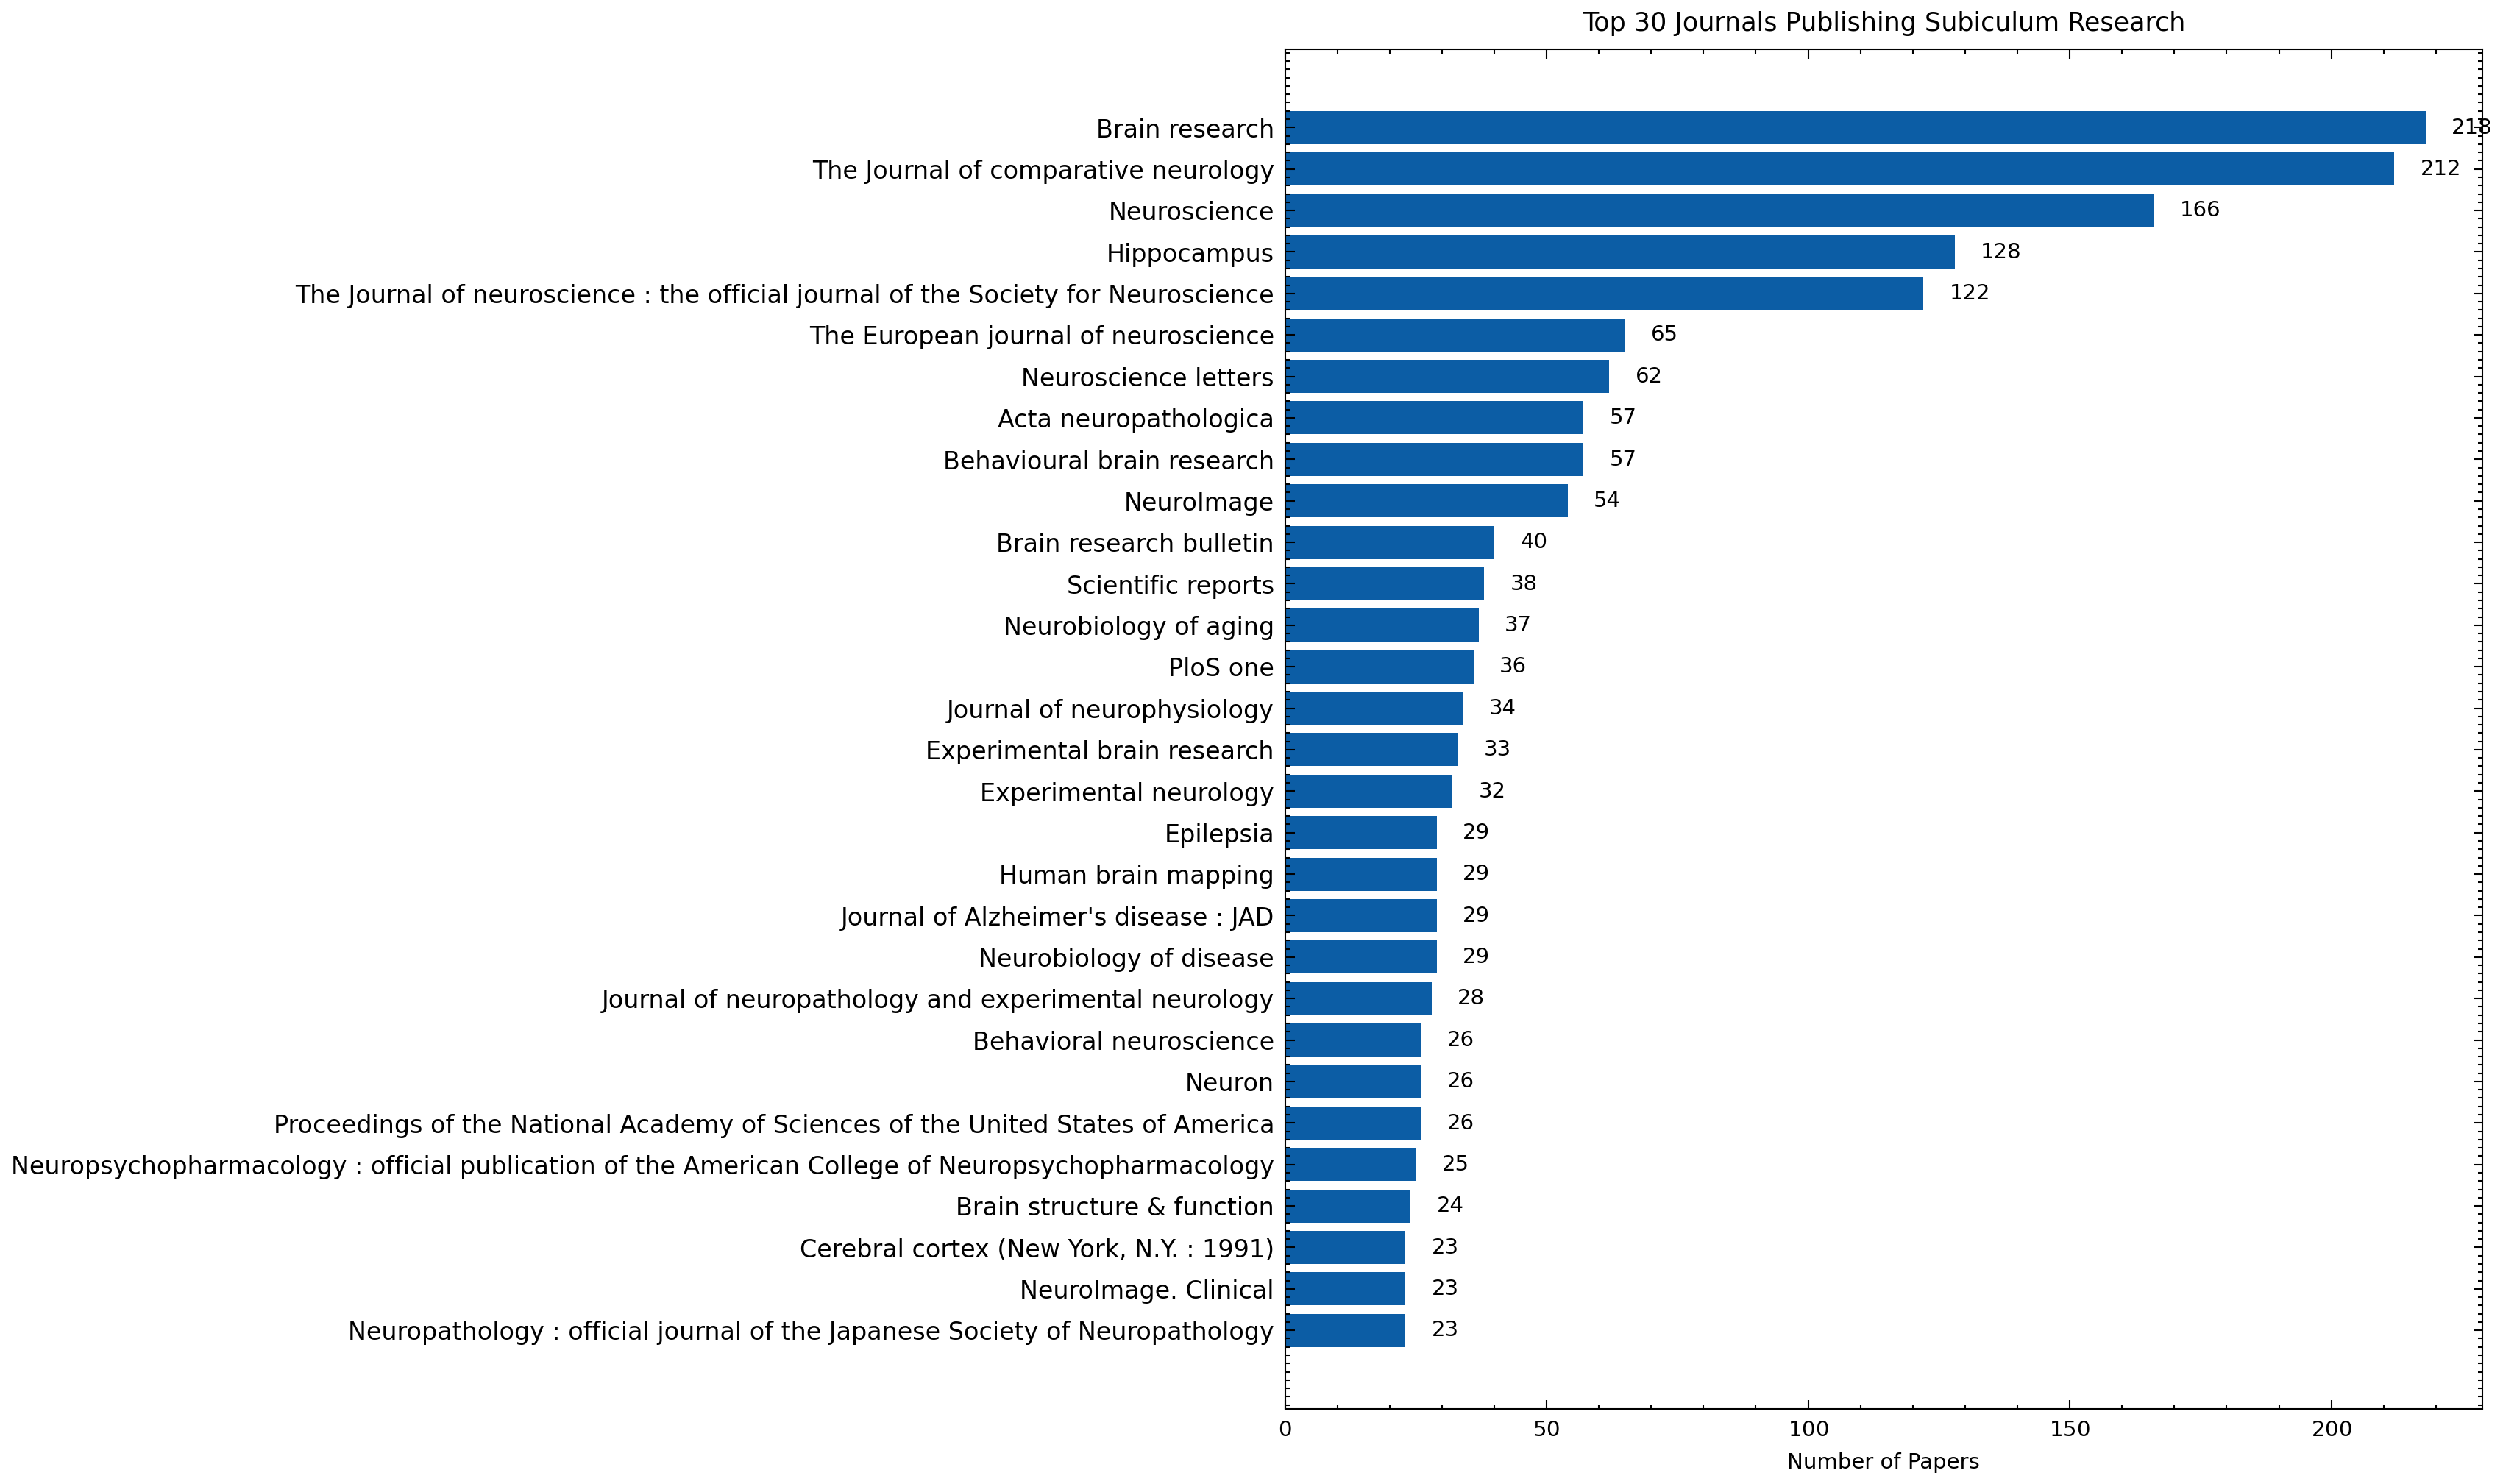
\includegraphics[width=0.9\textwidth]{imgs/general_eda_2025-12-06_top_journals.png}
\caption{Top 30 journals publishing subiculum research, showing strong concentration in core neuroscience venues.}
\label{fig:journals}
\end{figure}

\section{Author Contributions}

\subsection{Most Prolific Authors}

The analysis identified 15,603 unique authors contributing to subiculum research.

\begin{table}[htbp]
\centering
\caption{Top 5 most prolific authors in subiculum research}
\label{tab:authors}
\begin{tabular}{rlrrr}
\toprule
\textbf{Rank} & \textbf{Author} & \textbf{Papers} & \textbf{Career Span} & \textbf{Years Active} \\
\midrule
1 & Aggleton, John P & 27 & 2002--2024 & 22 years \\
2 & Witter, M P & 25 & 1982--2020 & 38 years \\
3 & Heinemann, U & 24 & 1986--2015 & 29 years \\
4 & Thompson, Paul M & 22 & 2003--2023 & 20 years \\
5 & Grace, Anthony A & 20 & 2005--2022 & 17 years \\
\bottomrule
\end{tabular}
\end{table}

\textbf{Note:} 83.3\% (12,998 out of 15,603 authors) appear on only one paper in the database.

\begin{table}[htbp]
\centering
\caption{Author contribution tiers}
\label{tab:author_tiers}
\begin{tabular}{lrr}
\toprule
\textbf{Author Tier} & \textbf{Count} & \textbf{\% of Total} \\
\midrule
1 paper only & 12,998 & 83.3\% \\
2--5 papers & 2,439 & 15.6\% \\
6--10 papers & 144 & 0.9\% \\
11+ papers (core) & 22 & 0.1\% \\
\bottomrule
\end{tabular}
\end{table}

Key insights:
\begin{itemize}[noitemsep]
    \item Core contributors: Only 22 authors (0.1\%) have published 11+ papers on subiculum
    \item Regular contributors: 144 authors (0.9\%) have 6--10 papers (see Appendix \ref{app:contributors})
    \item Long tail: A vast majority (83\%) are ``one-time'' contributors
\end{itemize}

\subsection{Collaboration Patterns}

\begin{itemize}[noitemsep]
    \item Single-author papers: 171 (4.8\%)
    \item Multi-author papers: 3,404 (95.2\%)
    \item Average authors per paper: 4.6 (increasing over time)
    \item Largest collaboration: 332 authors on a single paper
\end{itemize}

\begin{figure}[htbp]
\centering
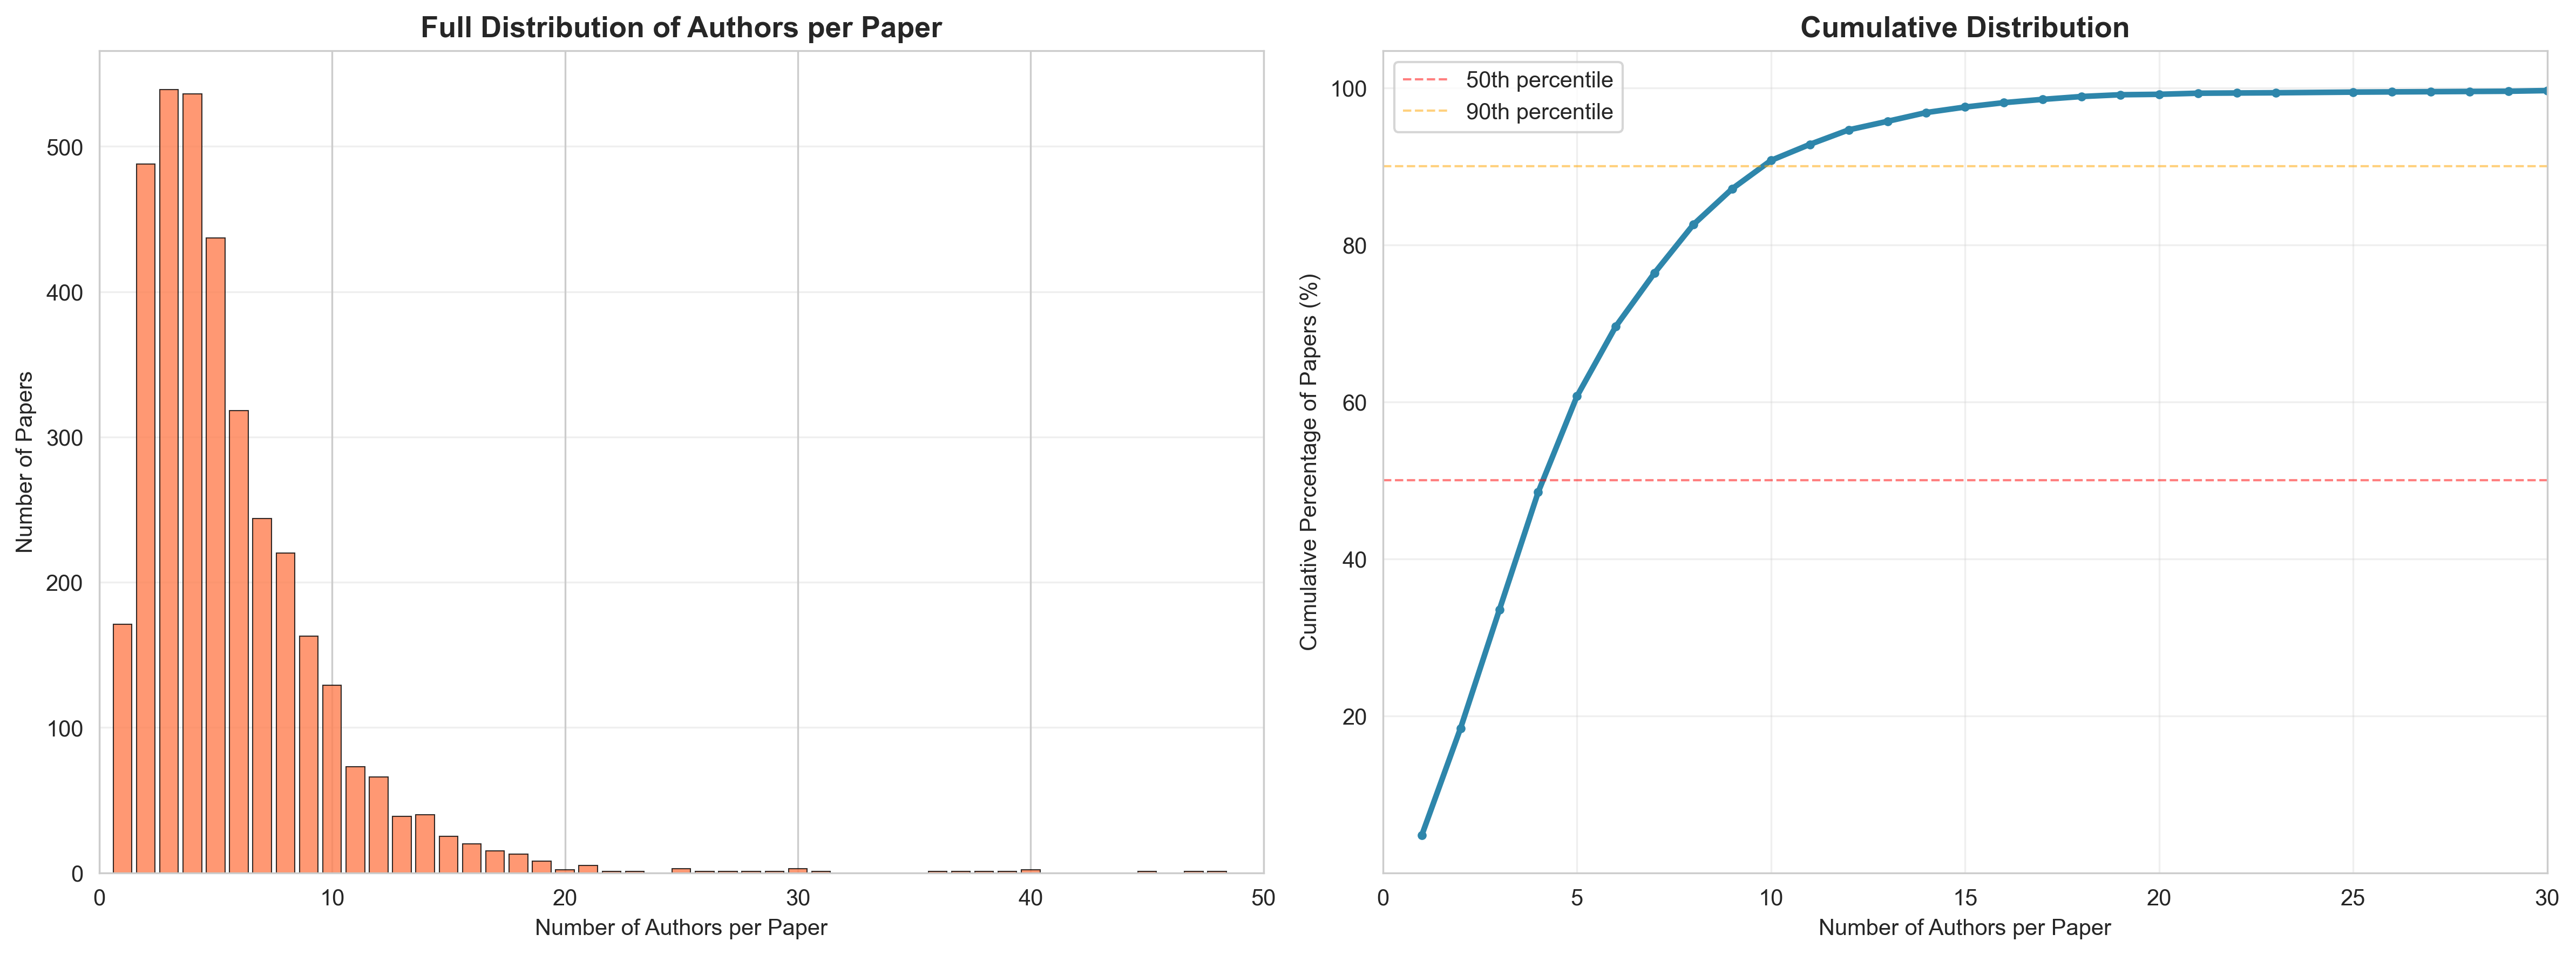
\includegraphics[width=\textwidth]{imgs/general_eda_2025-12-06_author_count_distribution.png}
\caption{Distribution of author counts per paper showing predominance of small collaborative teams (left) and cumulative distribution (right).}
\label{fig:author_dist}
\end{figure}

Collaboration has increased steadily, with the average number of authors per paper rising from approximately 2 in the 1970s to approximately 6 in the 2020s.

\begin{figure}[htbp]
\centering
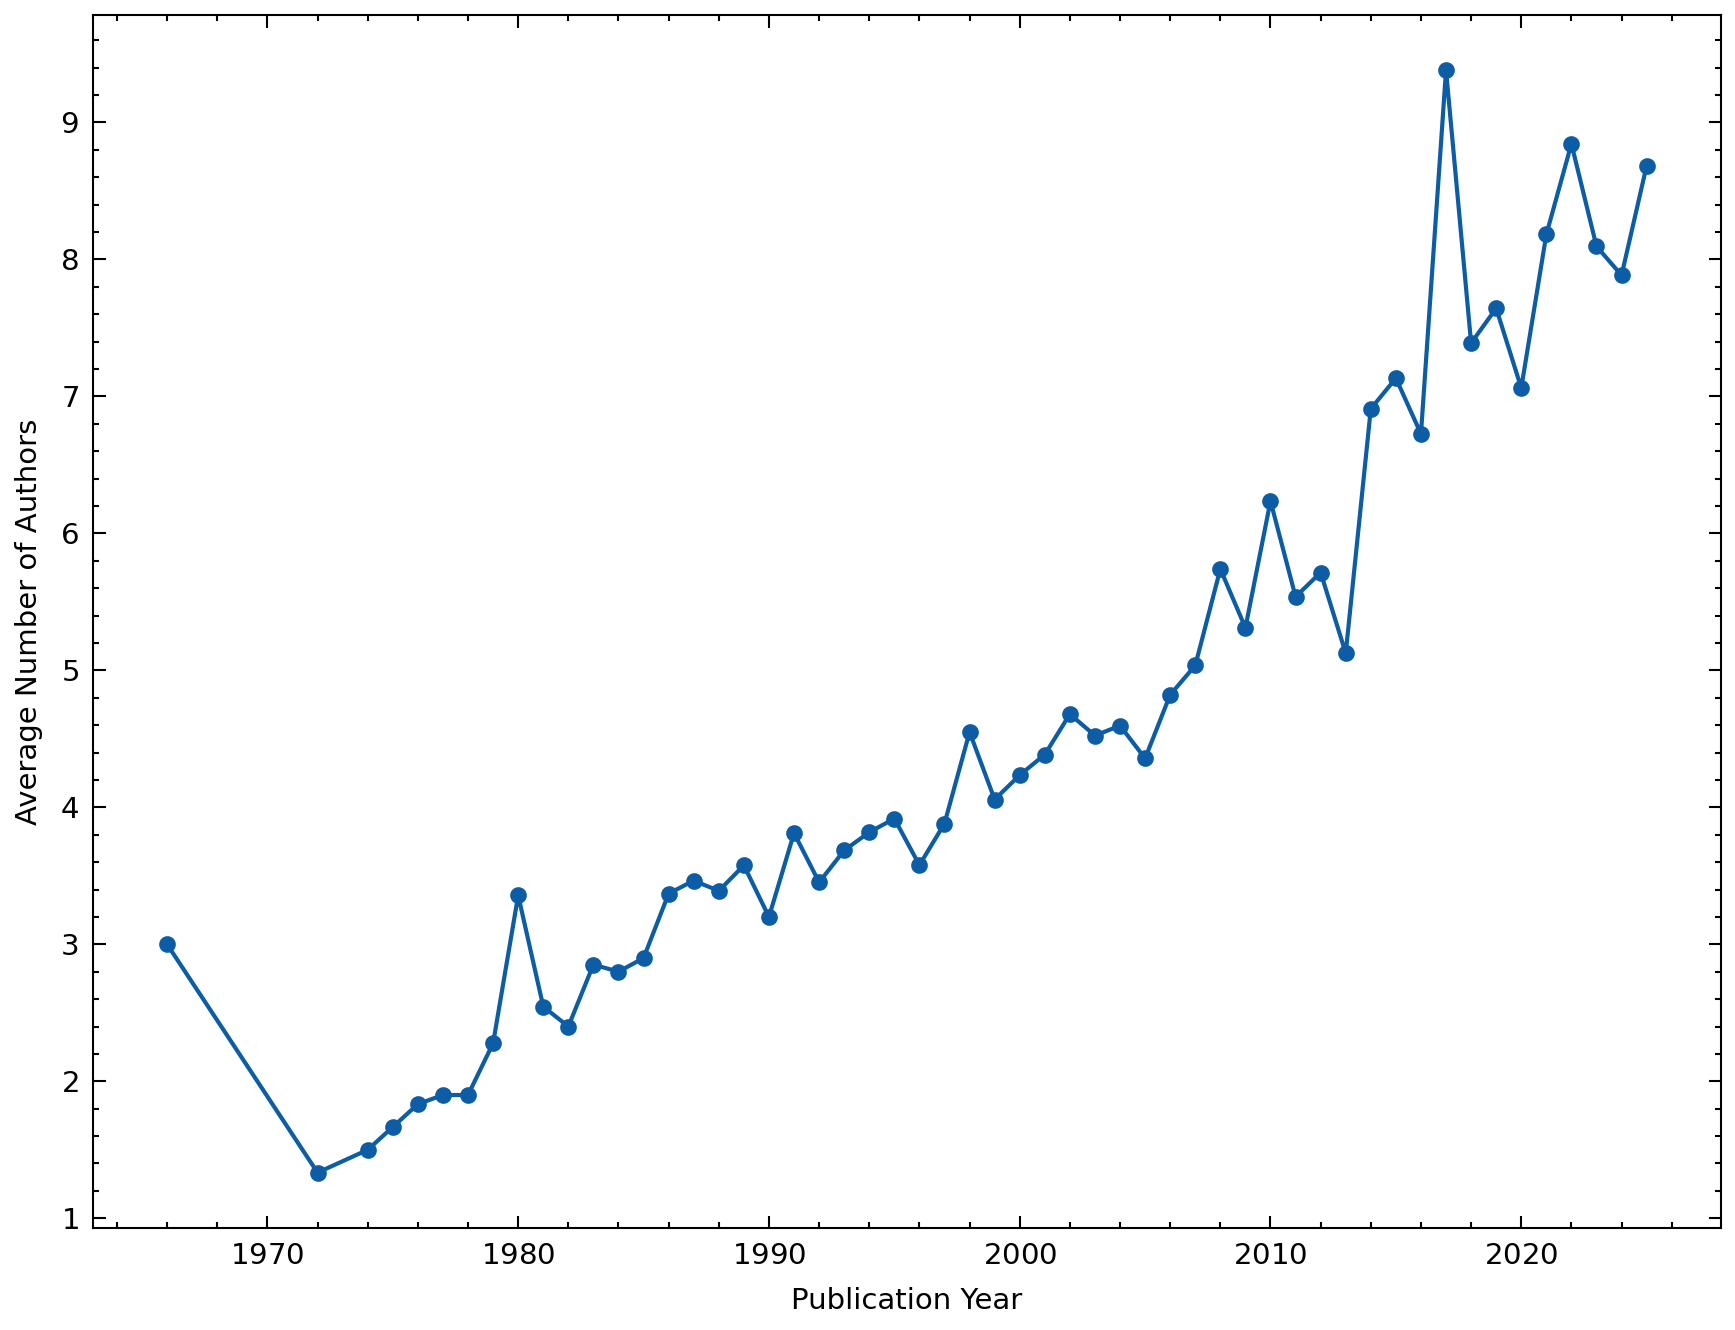
\includegraphics[width=0.8\textwidth]{imgs/general_eda_2025-12-06_avg_authors_over_time.png}
\caption{Average number of authors per paper over time, showing steady increase in collaboration.}
\label{fig:authors_time}
\end{figure}

\section{Citation Network Analysis}

\subsection{Citation Coverage}

Citation enrichment via CrossRef and Semantic Scholar achieved:
\begin{itemize}[noitemsep]
    \item 2,874 papers with reference lists (80.4\%)
    \item 98,445 total citation links
    \item Average 34.3 references per paper (for papers with citations)
\end{itemize}

\subsection{Most Influential Papers}

\begin{table}[htbp]
\centering
\caption{Top 5 most cited papers in the dataset}
\label{tab:cited}
\small
\begin{tabular}{lp{5cm}rp{3cm}}
\toprule
\textbf{PMID} & \textbf{Title (Year)} & \textbf{Cited} & \textbf{Journal} \\
\midrule
65364 & An autoradiographic study... (1977) & 220 & J. Comp. Neurol. \\
11240210 & The subiculum: a review... (2001) & 160 & Prog. Neurobiol. \\
16185252 & The subiculum: what it does... (2005) & 114 & J. Anatomy \\
1727001 & Organization of CA1 projections... (1991) & 110 & Hippocampus \\
3683859 & Organization of projections... (1987) & 109 & Neuroscience \\
\bottomrule
\end{tabular}
\end{table}

\textbf{Classic paper:} The most cited work (PMID 65364, 1977) remains foundational after 48 years, demonstrating the enduring importance of early neuroanatomical studies.

\begin{figure}[htbp]
\centering
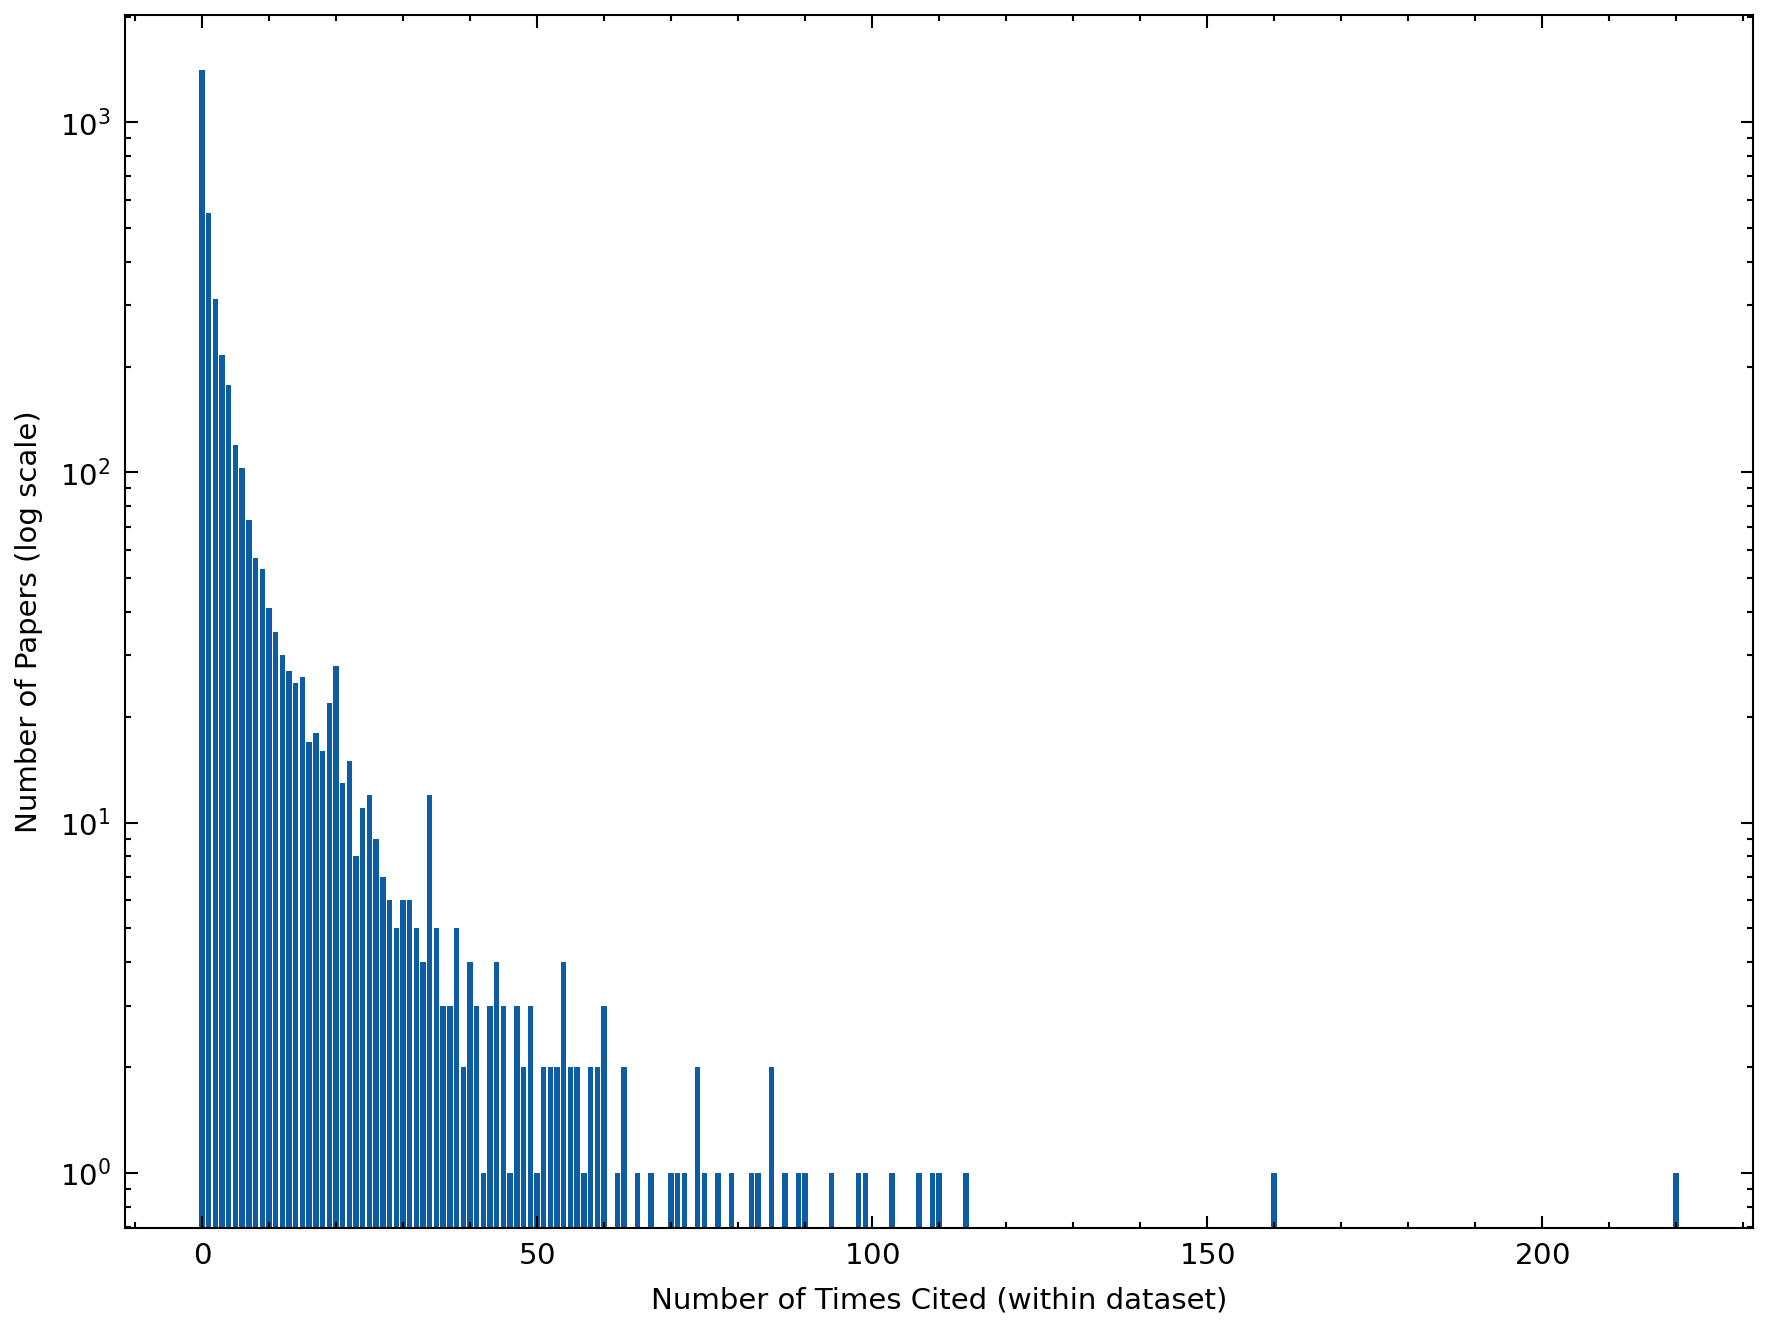
\includegraphics[width=0.8\textwidth]{imgs/general_eda_2025-12-06_citation_distribution.png}
\caption{Citation distribution showing typical long-tail pattern with few highly-cited papers and many with few citations.}
\label{fig:citations}
\end{figure}

\subsection{Citation Coverage by Era}

Recent papers have excellent citation coverage, while pre-2000 papers show gaps that may require additional enrichment from historical databases.

\begin{table}[htbp]
\centering
\caption{Citation coverage by decade}
\label{tab:citation_era}
\begin{tabular}{lr}
\toprule
\textbf{Decade} & \textbf{Citation Coverage} \\
\midrule
1960s--1970s & 45.5\% \\
1980s--1990s & 63.5\% \\
2000s & 72.7\% \\
2010s & 92.5\% \\
2020s & 97.4\% \\
\bottomrule
\end{tabular}
\end{table}

\section{Research Themes}

\subsection{MeSH Term Analysis}

\textbf{Coverage:} 91.2\% of papers (3,262/3,576) have MeSH annotations.

Top 10 MeSH terms reveal core research domains, with hippocampus and animal models dominating, alongside significant human and clinical research focus on aging and Alzheimer's disease.

\begin{table}[htbp]
\centering
\caption{Top 10 MeSH terms in the dataset}
\label{tab:mesh}
\begin{tabular}{lrr}
\toprule
\textbf{MeSH Term} & \textbf{Papers} & \textbf{\% of Dataset} \\
\midrule
Hippocampus & 2,330 & 65.2\% \\
Animals & 2,118 & 59.2\% \\
Male & 2,059 & 57.6\% \\
Female & 1,243 & 34.8\% \\
Humans & 1,379 & 38.6\% \\
Rats & 1,287 & 36.0\% \\
Neurons & 764 & 21.4\% \\
Aged & 594 & 16.6\% \\
Brain & 593 & 16.6\% \\
MRI & 560 & 15.7\% \\
Alzheimer Disease & 460 & 12.9\% \\
\bottomrule
\end{tabular}
\end{table}

\begin{figure}[htbp]
\centering
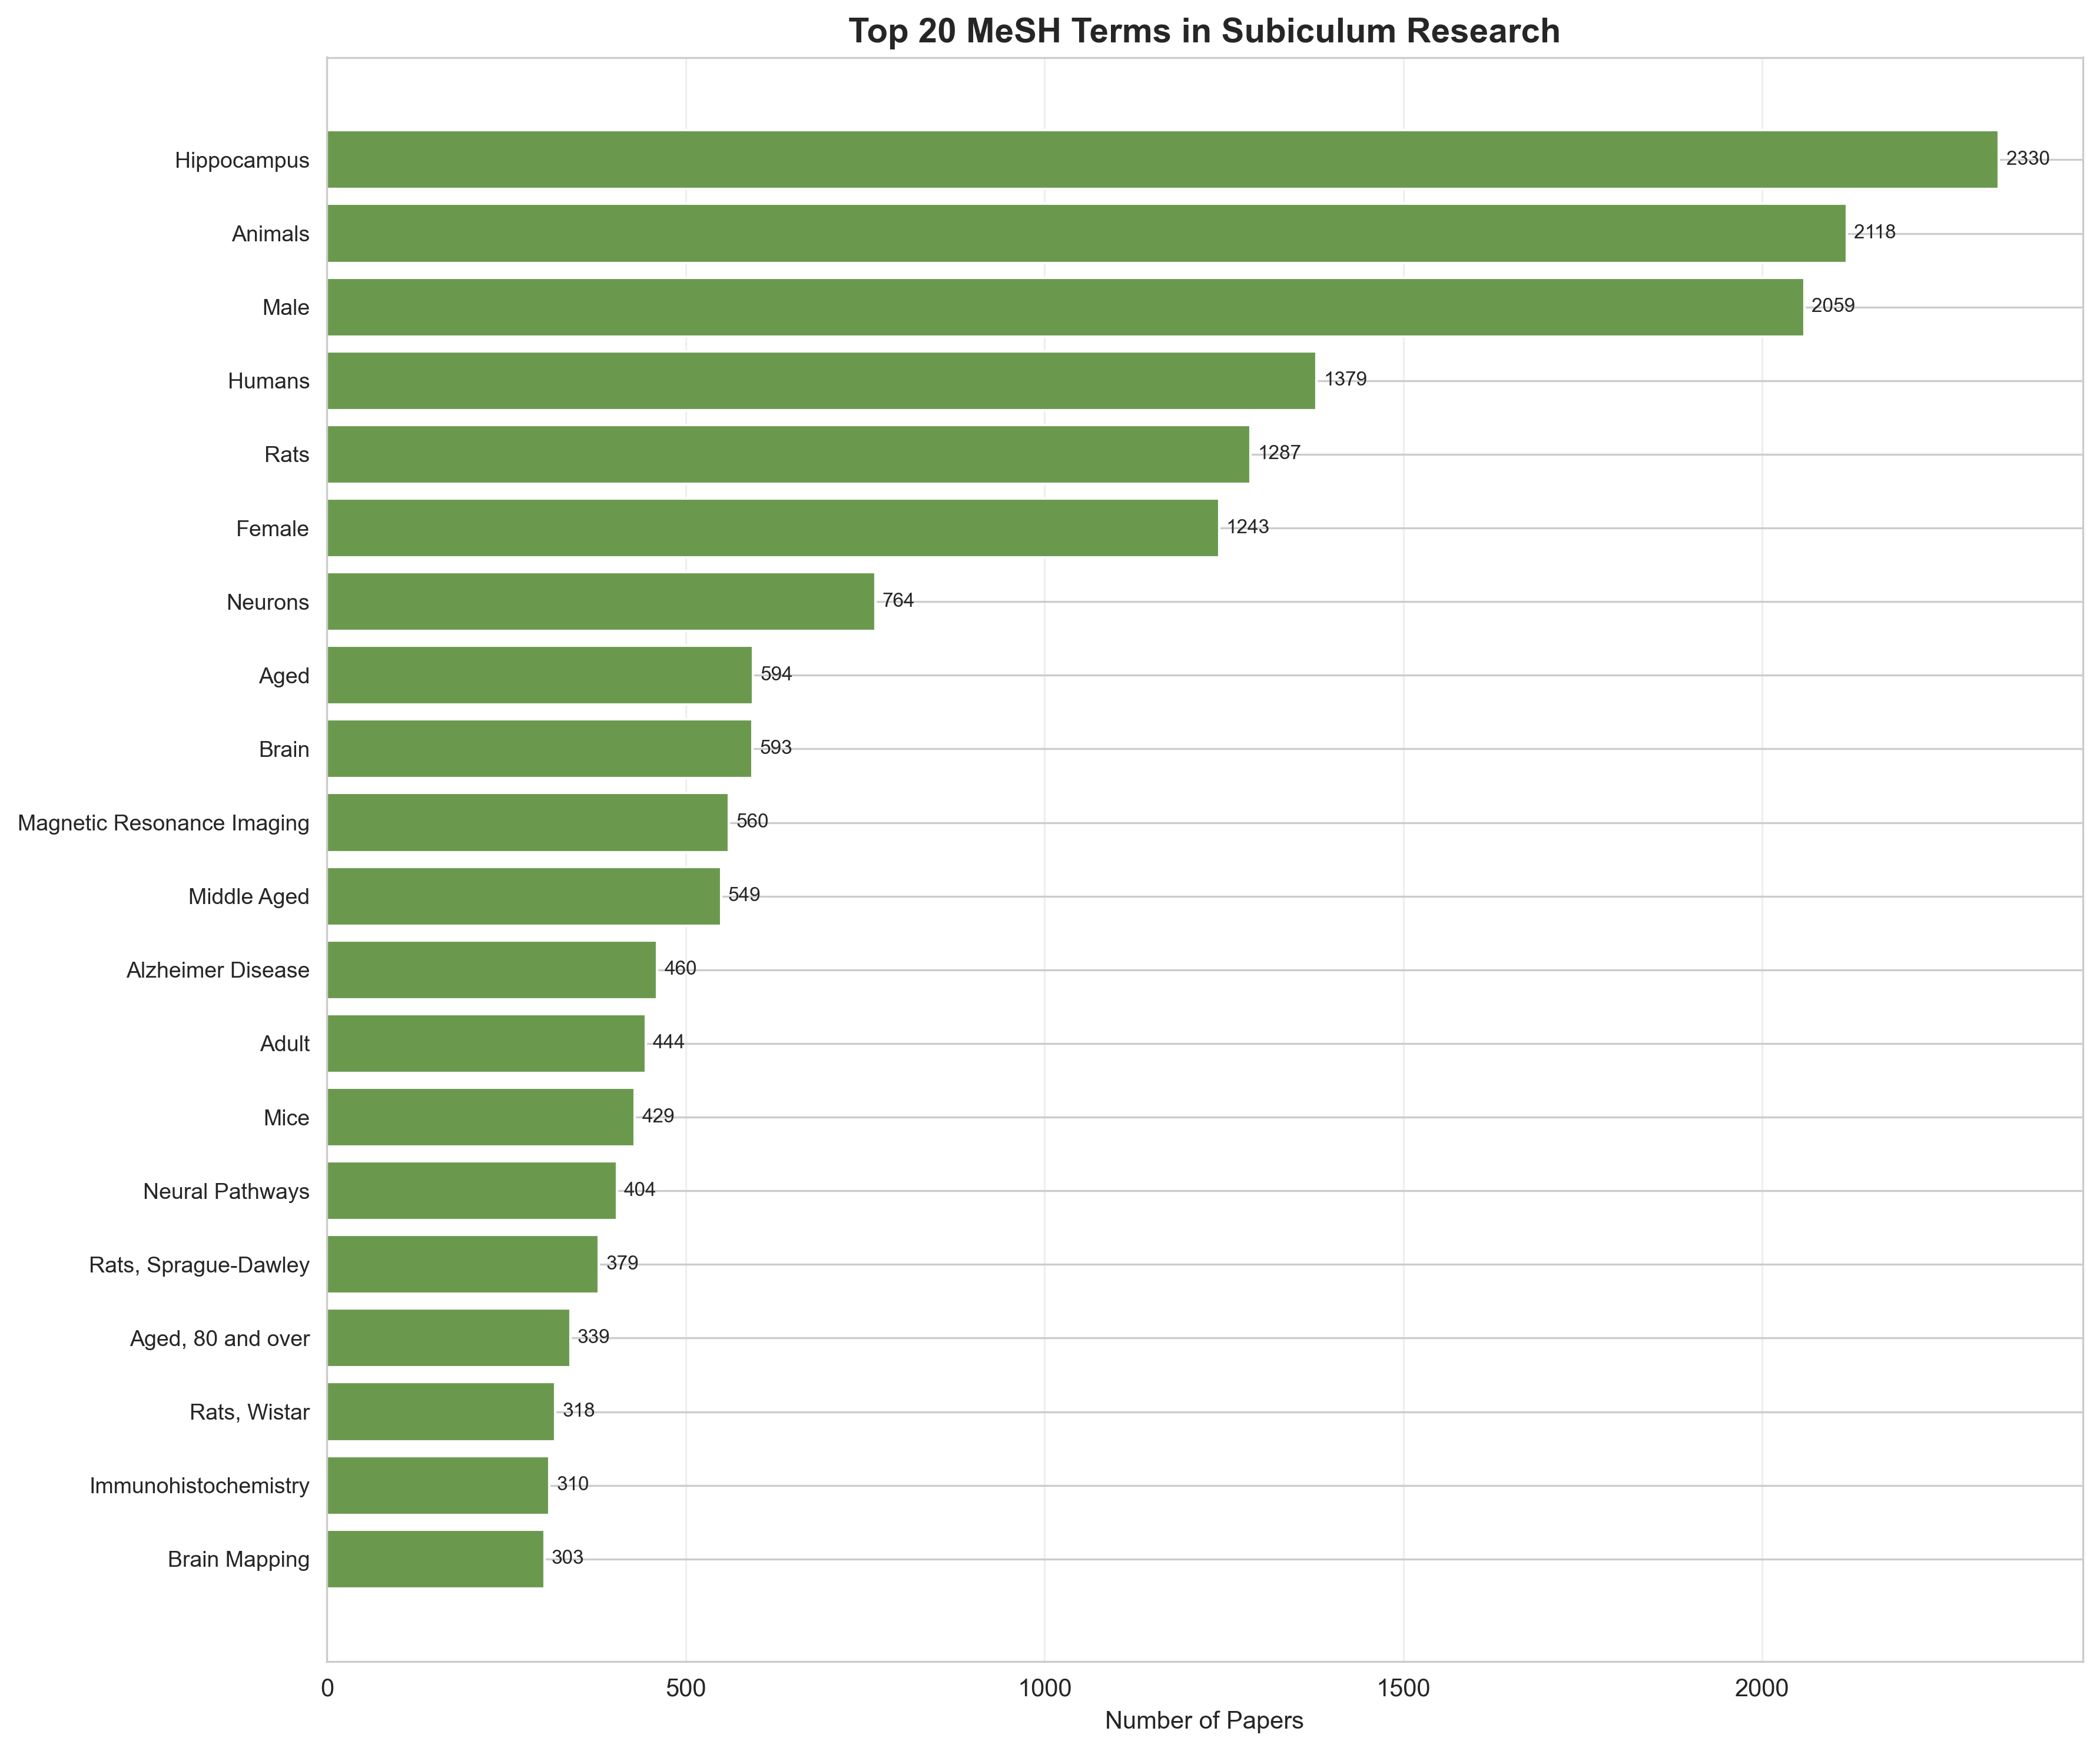
\includegraphics[width=0.9\textwidth]{imgs/general_eda_2025-12-06_top_mesh_terms.png}
\caption{Top 20 MeSH terms showing dominance of neuroanatomical and disease-focused research.}
\label{fig:mesh}
\end{figure}

\textbf{Key Insight:} The predominance of animal models (59\%) alongside human studies (39\%) reflects the field's dual focus on basic neuroscience and clinical translation. Alzheimer's disease represents the largest disease-specific research area.

\subsection{Author Keywords}

\textbf{Coverage:} 35\% of papers (1,250/3,576) include author-assigned keywords.

Top author-provided keywords show research focus areas: hippocampus (305 papers), subiculum (146 papers), Alzheimer's disease (105 papers), MRI (67 papers), and hippocampal subfields (57 papers).

\textbf{Note:} MeSH terms provide more comprehensive semantic coverage (91\%) than author keywords (35\%), making them preferable for topic modeling.

\section{Publication Types}

The dataset is dominated by primary research articles, with over 50\% of papers acknowledging external research support and NIH funding appearing in approximately 28\% of papers.

\begin{table}[htbp]
\centering
\caption{Distribution of publication types}
\label{tab:pubtypes}
\begin{tabular}{lrr}
\toprule
\textbf{Publication Type} & \textbf{Count} & \textbf{\% of Total} \\
\midrule
Journal Article & 3,569 & 99.8\% \\
Research Support, Non-U.S. Gov't & 1,853 & 51.8\% \\
Research Support, U.S. Gov't, P.H.S. & 510 & 14.3\% \\
Research Support, N.I.H., Extramural & 485 & 13.6\% \\
Comparative Study & 293 & 8.2\% \\
Review & 136 & 3.8\% \\
Case Reports & 51 & 1.4\% \\
Preprint & 25 & 0.7\% \\
\bottomrule
\end{tabular}
\end{table}

\begin{figure}[htbp]
\centering
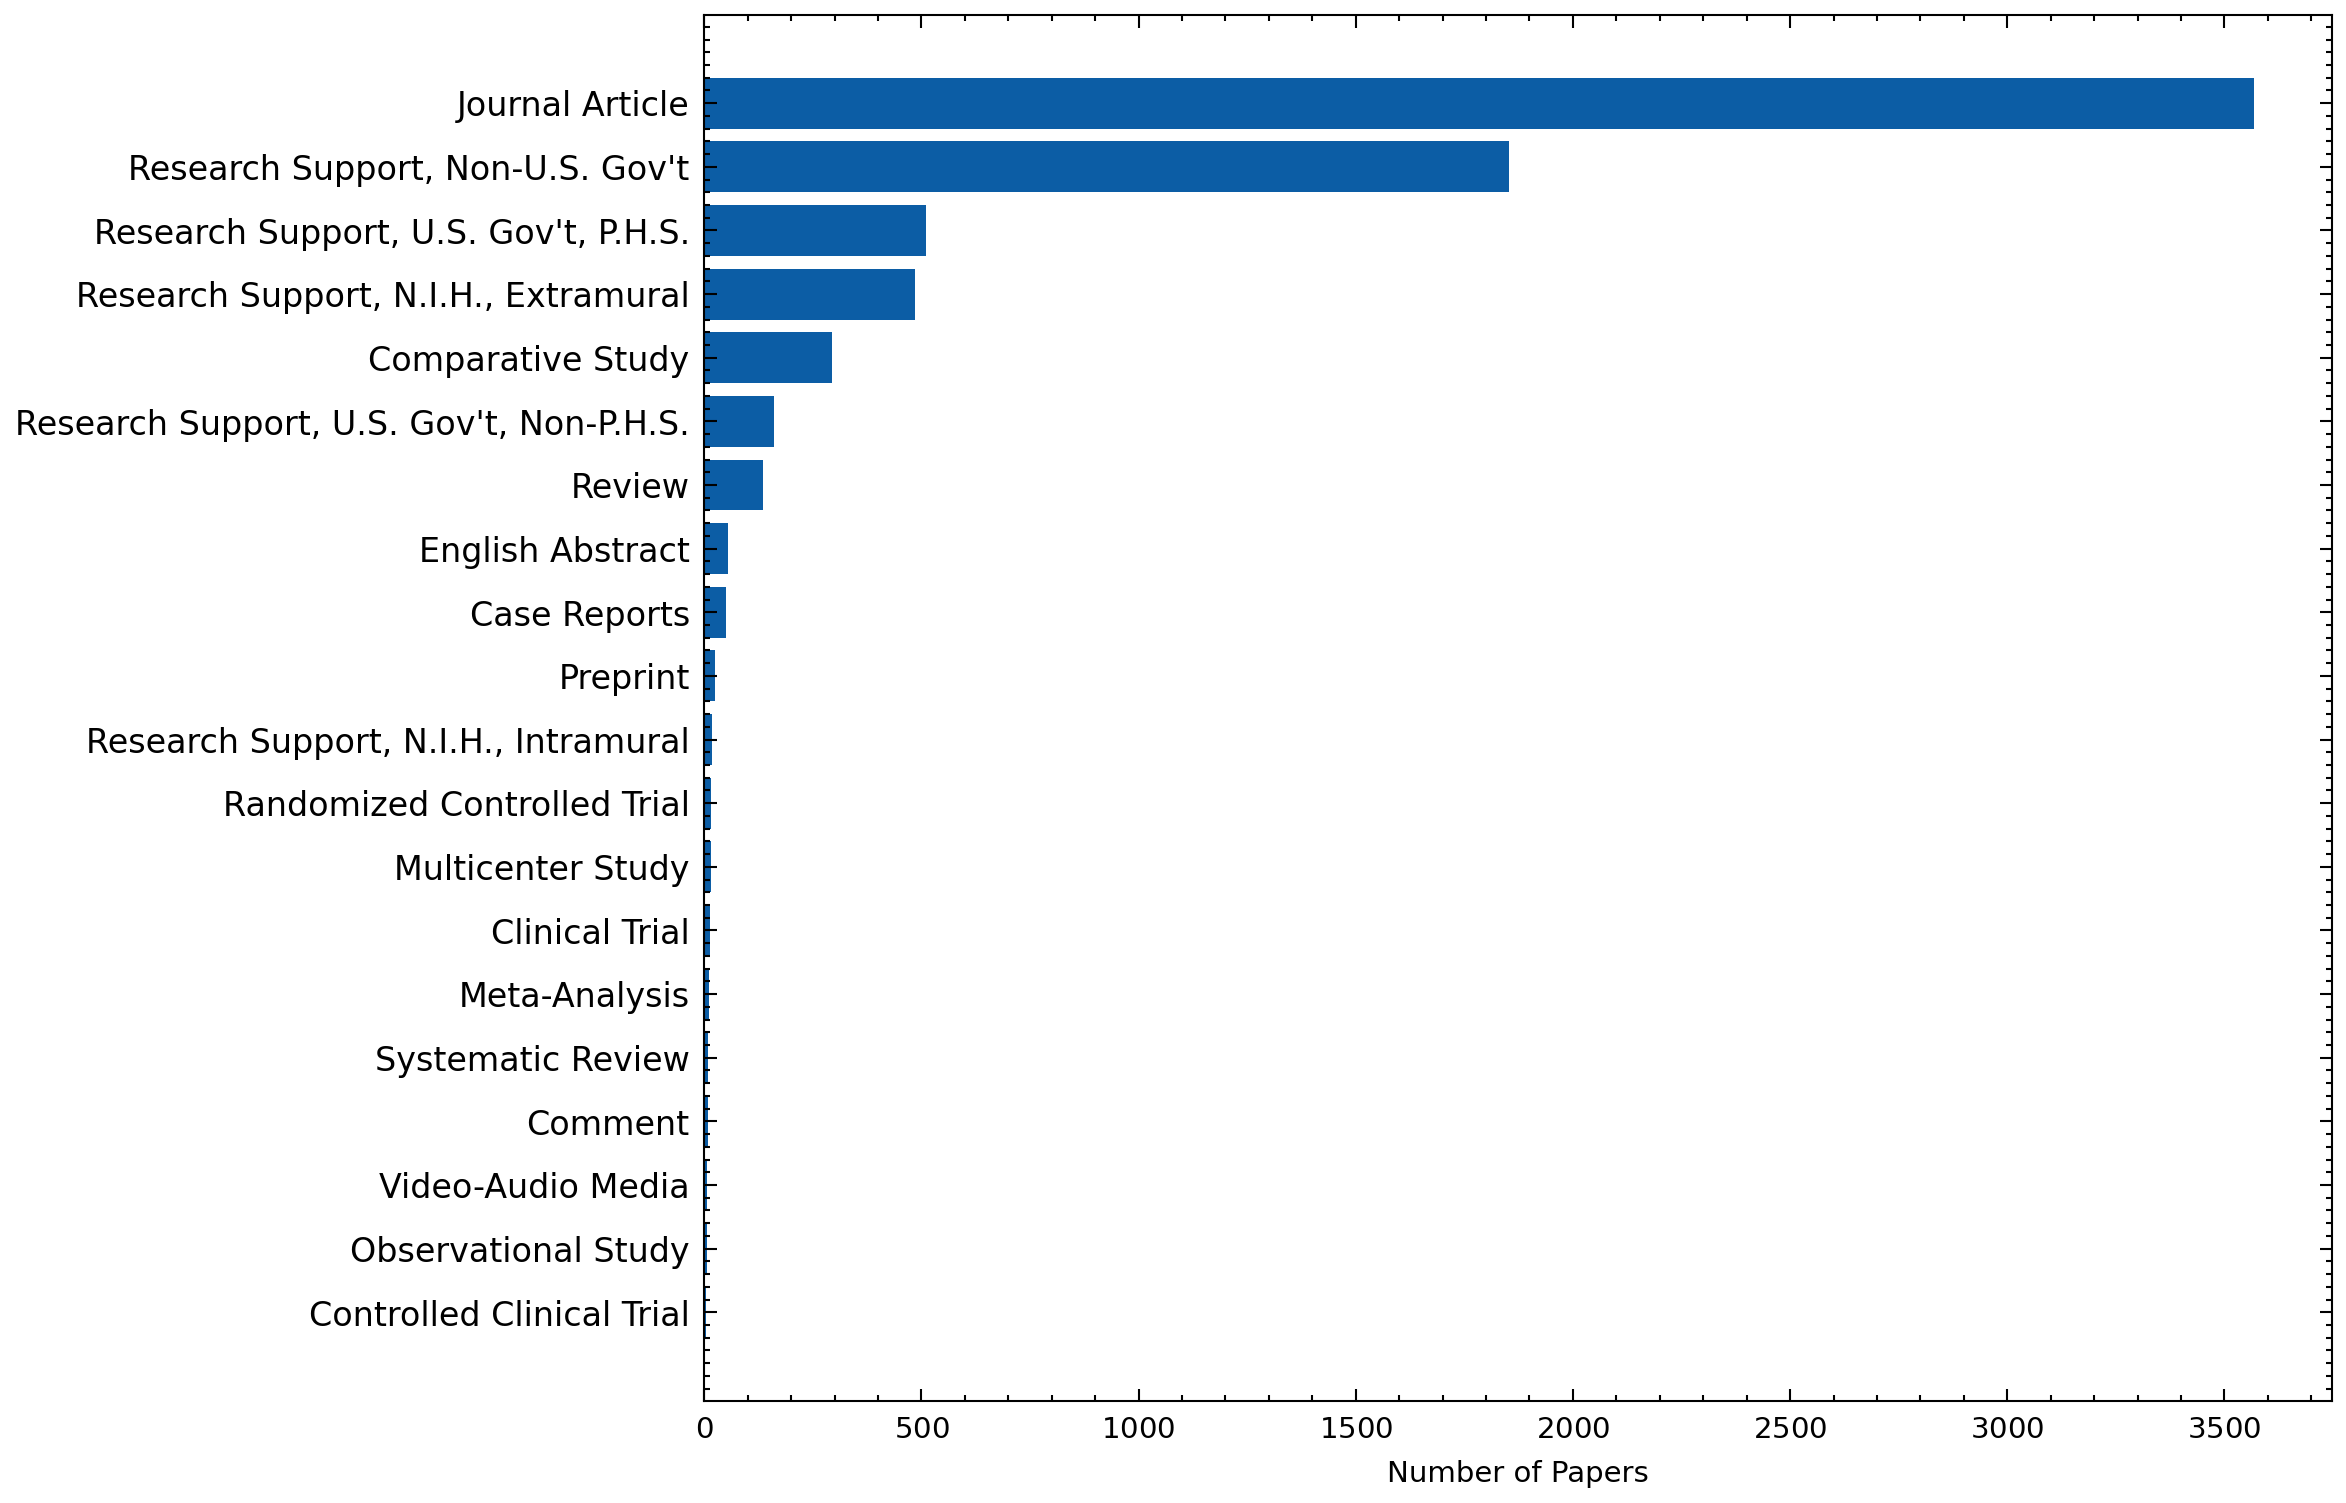
\includegraphics[width=0.9\textwidth]{imgs/general_eda_2025-12-06_publication_types.png}
\caption{Publication type distribution showing dominance of research articles with significant funding support.}
\label{fig:pubtypes}
\end{figure}

\section{Data Quality Assessment}

The dataset exhibits excellent metadata quality, with greater than 95\% completeness for core bibliographic fields.

\begin{table}[htbp]
\centering
\caption{Metadata completeness summary}
\label{tab:quality}
\begin{tabular}{lr}
\toprule
\textbf{Field} & \textbf{Completeness} \\
\midrule
Title & 100\% \\
Journal & 100\% \\
Year & 99.9\% \\
Abstract & 99.1\% \\
DOI & 95.7\% \\
PMC ID & 39.7\% \\
\bottomrule
\end{tabular}
\end{table}

\section{Key Takeaways}

\subsection{Research Landscape}
\begin{enumerate}[noitemsep]
    \item \textbf{Accelerating field:} 39\% of all subiculum research published in last 10 years
    \item \textbf{Interdisciplinary:} Spans neuroscience, neuroimaging, psychiatry, and aging research
    \item \textbf{Well-documented:} 91\% MeSH coverage enables semantic analysis
    \item \textbf{Collaborative:} Average 4.6 authors per paper, increasing over time
\end{enumerate}

\subsection{Dominant Themes}
\begin{enumerate}[noitemsep]
    \item \textbf{Neuroanatomy \& Connectivity:} Foundation of the field (1970s--1990s classics)
    \item \textbf{Alzheimer's Disease:} Largest clinical application (460 papers, 12.9\%)
    \item \textbf{Neuroimaging:} Methodological evolution (MRI: 560 papers, 15.7\%)
    \item \textbf{Animal Models:} Predominantly rodent studies (59\% of papers)
\end{enumerate}

\subsection{Data Strengths}
\begin{itemize}[noitemsep]
    \item Comprehensive temporal coverage (59 years)
    \item High metadata quality (>95\% completeness)
    \item Rich semantic annotations (91\% MeSH terms)
    \item Strong citation network (80\% coverage)
\end{itemize}

\subsection{Data Limitations}
\begin{itemize}[noitemsep]
    \item Pre-2000 citation data incomplete (45--65\% coverage)
    \item Author keywords sparse (35\% of papers)
    \item Limited to PubMed-indexed literature (excludes books, dissertations)
\end{itemize}

\section{Future Directions}

\subsection{For Literature Review}
\begin{itemize}[noitemsep]
    \item Focus on 2010+ papers for best citation coverage
    \item Prioritize MeSH terms over author keywords for topic modeling
    \item Consider top 10 journals for comprehensive coverage (32\% of literature)
\end{itemize}

\subsection{For Citation Analysis}
\begin{itemize}[noitemsep]
    \item Supplement pre-2000 papers with Web of Science or Scopus
    \item Strong foundation in comparative neuroanatomy
\end{itemize}

\subsection{For Bibliometric Analysis}
\begin{itemize}[noitemsep]
    \item Collaboration networks show increasing complexity over time
    \item NIH-funded research represents core of U.S. contributions
    \item European Journal of Neuroscience represents major international venue
\end{itemize}

\appendix

\clearpage
\section{Regular Contributors (6--10 Papers)}
\label{app:contributors}

This appendix provides a complete list of all 144 authors who have published 6--10 papers on subiculum research. These regular contributors represent 0.9\% of all authors but have sustained engagement with the field over multiple years.

\begin{longtable}{lrrrr}
\caption{Complete list of regular contributors (6--10 papers)} \label{tab:regular-contributors} \\
\toprule
\textbf{Author} & \textbf{Papers} & \textbf{First Pub} & \textbf{Latest Pub} & \textbf{Years Active} \\
\midrule
\endfirsthead

\multicolumn{5}{c}{\tablename\ \thetable\ -- \textit{Continued from previous page}} \\
\toprule
\textbf{Author} & \textbf{Papers} & \textbf{First Pub} & \textbf{Latest Pub} & \textbf{Years Active} \\
\midrule
\endhead

\midrule
\multicolumn{5}{r}{\textit{Continued on next page}} \\
\endfoot

\bottomrule
\endlastfoot

Wozny, Christian & 10 & 2005 & 2025 & 20 \\
Raz, Naftali & 10 & 2011 & 2025 & 14 \\
Wang, Yi & 10 & 2012 & 2025 & 13 \\
Vann, Seralynne D & 10 & 2005 & 2022 & 17 \\
Spruston, Nelson & 10 & 2003 & 2019 & 16 \\
Lévesque, Maxime & 10 & 2011 & 2018 & 7 \\
Miles, Richard & 10 & 2002 & 2016 & 14 \\
Rawlins, J N & 10 & 1986 & 2001 & 15 \\
Hyman, B T & 10 & 1984 & 1998 & 14 \\
Jarrard, L E & 10 & 1978 & 1997 & 19 \\
Tohyama, M & 10 & 1980 & 1993 & 13 \\
de Flores, Robin & 9 & 2015 & 2025 & 10 \\
Ding, Song-Lin & 9 & 2007 & 2025 & 18 \\
Insausti, Ricardo & 9 & 2010 & 2025 & 15 \\
Fei, Fan & 9 & 2021 & 2025 & 4 \\
Mukherjee, Jogeshwar & 9 & 2006 & 2025 & 19 \\
Chen, Zhong & 9 & 2019 & 2025 & 6 \\
Chételat, Gaël & 9 & 2010 & 2025 & 15 \\
Chakravarty, M Mallar & 9 & 2013 & 2025 & 12 \\
Jack, Clifford R & 9 & 2006 & 2024 & 18 \\
Whitwell, Jennifer L & 9 & 2006 & 2024 & 18 \\
Amin, Eman & 9 & 2003 & 2024 & 21 \\
Wisse, Laura E M & 9 & 2014 & 2023 & 9 \\
Sperk, Günther & 9 & 2003 & 2022 & 19 \\
Kutty, Bindu M & 9 & 2003 & 2022 & 19 \\
Toga, Arthur W & 9 & 2006 & 2017 & 11 \\
O'Mara, S M & 9 & 1998 & 2017 & 19 \\
Lopes da Silva, F H & 9 & 1982 & 2009 & 27 \\
Wouterlood, F G & 9 & 1990 & 2008 & 18 \\
Totterdell, S & 9 & 1986 & 2005 & 19 \\
Hof, P R & 9 & 1987 & 2002 & 15 \\
West, M J & 9 & 1984 & 2001 & 17 \\
Gloveli, T & 9 & 1994 & 2001 & 7 \\
Wyss, J M & 9 & 1983 & 1999 & 16 \\
Yanagihara, T & 9 & 1985 & 1995 & 10 \\
Chan-Palay, V & 9 & 1981 & 1988 & 7 \\
Uemura, E & 9 & 1979 & 1985 & 6 \\
Moon, Minho & 8 & 2012 & 2025 & 13 \\
Huang, Yushan & 8 & 2015 & 2025 & 10 \\
Petersen, Ronald C & 8 & 2006 & 2024 & 18 \\
Josephs, Keith A & 8 & 2006 & 2024 & 18 \\
Drexel, Meinrad & 8 & 2012 & 2023 & 11 \\
Schmitz, Dietmar & 8 & 2008 & 2021 & 13 \\
Miller, Michael I & 8 & 2003 & 2017 & 14 \\
Csernansky, John G & 8 & 2003 & 2016 & 13 \\
Stewart, M & 8 & 1997 & 2008 & 11 \\
Kawasaki, H & 8 & 1996 & 2007 & 11 \\
de Leon, M J & 8 & 1990 & 2002 & 12 \\
Harrison, P J & 8 & 1990 & 2001 & 11 \\
Feldon, J & 8 & 1986 & 2000 & 14 \\
Price, J L & 8 & 1974 & 1999 & 25 \\
McEwen, B S & 8 & 1982 & 1998 & 16 \\
Cotman, C W & 8 & 1986 & 1997 & 11 \\
Bossert, Jennifer M & 7 & 2013 & 2025 & 12 \\
Landeau, Brigitte & 7 & 2010 & 2025 & 15 \\
Saunders, Richard C & 7 & 2002 & 2024 & 22 \\
Joksimovic, Srdjan M & 7 & 2017 & 2023 & 6 \\
Zeineh, Michael M & 7 & 2003 & 2021 & 18 \\
Anderson, M & 7 & 1998 & 2020 & 22 \\
Herman, James P & 7 & 2002 & 2018 & 16 \\
Apostolova, Liana G & 7 & 2006 & 2017 & 11 \\
Cooper, Donald C & 7 & 2002 & 2013 & 11 \\
Raju, T R & 7 & 1997 & 2011 & 14 \\
Gonzalez-Lima, F & 7 & 1994 & 2011 & 17 \\
Arnold, S E & 7 & 1991 & 2007 & 16 \\
Pitkänen, A & 7 & 1992 & 2004 & 12 \\
Armstrong, D M & 7 & 1988 & 2003 & 15 \\
Yee, B K & 7 & 1995 & 2002 & 7 \\
Bouras, C & 7 & 1994 & 2002 & 8 \\
Morrison, J H & 7 & 1988 & 2002 & 14 \\
Commins, S & 7 & 1998 & 2001 & 3 \\
Gray, J A & 7 & 1985 & 2001 & 16 \\
Joyce, J N & 7 & 1989 & 2000 & 11 \\
Geneser, F A & 7 & 1987 & 1997 & 10 \\
Zimmer, J & 7 & 1978 & 1996 & 18 \\
Gessi, T & 7 & 1979 & 1995 & 16 \\
Siesjö, B K & 7 & 1984 & 1995 & 11 \\
Bennett, David A & 6 & 2003 & 2025 & 22 \\
Riggins, Tracy & 6 & 2018 & 2025 & 7 \\
Ofen, Noa & 6 & 2016 & 2025 & 9 \\
Liang, Christopher & 6 & 2023 & 2025 & 2 \\
Luders, Eileen & 6 & 2013 & 2025 & 12 \\
Kurth, Florian & 6 & 2013 & 2025 & 12 \\
Xu, Cenglin & 6 & 2017 & 2025 & 8 \\
Chen, Zhong & 6 & 2012 & 2025 & 13 \\
Wang, Yi & 6 & 2022 & 2025 & 3 \\
Mézenge, Florence & 6 & 2010 & 2025 & 15 \\
Waldvogel, Henry J & 6 & 2017 & 2025 & 8 \\
Lever, Colin & 6 & 2006 & 2025 & 19 \\
Gong, Qiyong & 6 & 2018 & 2025 & 7 \\
Wolk, David A & 6 & 2018 & 2025 & 7 \\
Xu, Xiangmin & 6 & 2014 & 2024 & 10 \\
La Joie, Renaud & 6 & 2010 & 2024 & 14 \\
Petrucelli, Leonard & 6 & 2014 & 2023 & 9 \\
Holmes, Todd C & 6 & 2016 & 2023 & 7 \\
Tesic, Vesna & 6 & 2019 & 2023 & 4 \\
Todorovic, Slobodan M & 6 & 2011 & 2023 & 12 \\
Veltman, Dick J & 6 & 2015 & 2023 & 8 \\
Honda, Yoshiko & 6 & 2004 & 2022 & 18 \\
Bender, Andrew R & 6 & 2013 & 2022 & 9 \\
Yoshida, Mari & 6 & 2009 & 2022 & 13 \\
Das, Sandhitsu R & 6 & 2010 & 2021 & 11 \\
Trojanowski, J Q & 6 & 1991 & 2021 & 30 \\
Tang, Xiaoying & 6 & 2015 & 2020 & 5 \\
Kinnavane, Lisa & 6 & 2016 & 2020 & 4 \\
Stark, Craig E L & 6 & 2008 & 2020 & 12 \\
Dillingham, Christopher M & 6 & 2015 & 2019 & 4 \\
Frisoni, Giovanni B & 6 & 2012 & 2019 & 7 \\
Somogyi, Peter & 6 & 2002 & 2018 & 16 \\
Argiolas, Antonio & 6 & 2009 & 2017 & 8 \\
Melis, Maria Rosaria & 6 & 2009 & 2017 & 8 \\
Gigg, John & 6 & 2006 & 2016 & 10 \\
Wright, Nicholas F & 6 & 2010 & 2016 & 6 \\
Ekstrom, Arne D & 6 & 2010 & 2015 & 5 \\
Bookheimer, Susan Y & 6 & 2003 & 2015 & 12 \\
Baulac, Michel & 6 & 2002 & 2015 & 13 \\
Akiyama, Haruhiko & 6 & 2002 & 2014 & 12 \\
Thom, M & 6 & 1997 & 2009 & 12 \\
Zilles, K & 6 & 1985 & 2005 & 20 \\
Eichenbaum, H & 6 & 1983 & 2005 & 22 \\
Bowery, N G & 6 & 1986 & 2003 & 17 \\
Ikonomovic, M D & 6 & 1995 & 2003 & 8 \\
van Groen, T & 6 & 1986 & 2003 & 17 \\
Wegiel, J & 6 & 1993 & 2002 & 9 \\
Vinogradova, O S & 6 & 1976 & 2001 & 25 \\
Yang, C R & 6 & 1984 & 2001 & 17 \\
Naber, P A & 6 & 1998 & 2001 & 3 \\
Ferrer, I & 6 & 1993 & 2001 & 8 \\
Greene, J R & 6 & 1996 & 2001 & 5 \\
Winblad, B & 6 & 1997 & 2000 & 3 \\
Bobinski, M & 6 & 1993 & 2000 & 7 \\
Wisniewski, H M & 6 & 1993 & 2000 & 7 \\
Berger, B & 6 & 1985 & 1999 & 14 \\
Moore, R Y & 6 & 1977 & 1997 & 20 \\
Slomianka, L & 6 & 1987 & 1997 & 10 \\
Hoyer, D & 6 & 1994 & 1996 & 2 \\
Gasbarri, A & 6 & 1989 & 1996 & 7 \\
Pacitti, C & 6 & 1989 & 1996 & 7 \\
Braak, H & 6 & 1972 & 1996 & 24 \\
Buzsáki, G & 6 & 1986 & 1994 & 8 \\
Vanderhaeghen, J J & 6 & 1989 & 1993 & 4 \\
Loy, R & 6 & 1979 & 1988 & 9 \\
Rainbow, T C & 6 & 1982 & 1985 & 3 \\
Siegel, A & 6 & 1977 & 1981 & 4 \\

\end{longtable}

\textbf{Notable contributors:}
\begin{itemize}[noitemsep]
    \item Trojanowski, J Q has the longest career span: 30 years (1991--2021)
    \item Vinogradova, O S started earliest (1976) with 25 years of contributions
    \item Braak, H published from 1972--1996 (24 years) -- important early Alzheimer's researcher
    \item Lopes da Silva, F H maintained 27 years of contributions (1982--2009)
\end{itemize}

\clearpage
\section{Data Files Reference}
\label{app:datafiles}

All analysis outputs are saved as CSV files in the \texttt{outputs/} directory with timestamp \texttt{2025-12-06}. The following files are referenced throughout this report:

\subsection{Core Dataset Files}
\begin{itemize}[noitemsep]
    \item \texttt{dataset\_overview.csv} -- Summary statistics of the complete dataset
    \item \texttt{data\_completeness.csv} -- Field-level completeness metrics
\end{itemize}

\subsection{Temporal Analysis}
\begin{itemize}[noitemsep]
    \item \texttt{papers\_by\_year.csv} -- Annual publication counts (1966--2025)
    \item \texttt{papers\_by\_decade.csv} -- Decadal aggregation of publications
\end{itemize}

\subsection{Publication Venues}
\begin{itemize}[noitemsep]
    \item \texttt{top\_journals.csv} -- Journal rankings by publication count
    \item \texttt{publication\_types.csv} -- Distribution of article types (research, review, etc.)
\end{itemize}

\subsection{Author Contributions}
\begin{itemize}[noitemsep]
    \item \texttt{top\_100\_authors.csv} -- Most prolific authors in subiculum research
\end{itemize}

\subsection{Citation Metrics}
\begin{itemize}[noitemsep]
    \item \texttt{most\_cited\_papers.csv} -- Highly cited papers in the dataset
    \item \texttt{citation\_distribution.csv} -- Distribution of citation counts across papers
\end{itemize}

\subsection{Research Themes}
\begin{itemize}[noitemsep]
    \item \texttt{top\_mesh\_terms.csv} -- Most frequent MeSH terms
    \item \texttt{top\_keywords.csv} -- Most frequent author-assigned keywords
\end{itemize}

\clearpage
\section{San Diego Institutional Contributions}
\label{app:sandiego}

San Diego area institutions represent less than 1\% of the dataset (33/3,576 papers, 0.9\%).

\begin{table}[htbp]
\centering
\caption{San Diego area institutional contributions}
\label{tab:sandiego-summary}
\begin{tabular}{lrr}
\toprule
\textbf{Institution} & \textbf{Papers} & \textbf{Authors} \\
\midrule
UCSD & 26 & 30+ \\
Salk Institute & 7 & 8 \\
Neurosciences Institute & 2 & 5 \\
\bottomrule
\end{tabular}
\end{table}

\textbf{UCSD Top Contributors:} Douglas Nitz (Cognitive Science) is the most prolific local contributor with 5 papers (2017-2025), focusing on spatial cognition and hippocampal subfield function. Recent work includes Alzheimer's disease research (Psychiatry), spatial coding (Cognitive Science), and developmental neuroscience (Neurosciences Department).

\textbf{Salk Institute:} Historical contributions in 1980s-1990s, with recent 2014-2015 systems neurobiology work. Notable: David Amaral (now at UC Davis) published from Salk in 1991; Edward Callaway is a prominent systems neuroscientist.

\subsection{Complete List of San Diego Papers}

\begin{longtable}{rp{6cm}lp{2.5cm}}
\caption{All papers with San Diego institutional affiliations (n=40)} \\
\toprule
\textbf{PMID} & \textbf{Title} & \textbf{Year} & \textbf{Authors} \\
\midrule
\endfirsthead

\multicolumn{4}{c}{\tablename\ \thetable\ -- \textit{Continued from previous page}} \\
\toprule
\textbf{PMID} & \textbf{Title} & \textbf{Year} & \textbf{Authors} \\
\midrule
\endhead

\midrule
\multicolumn{4}{r}{\textit{Continued on next page}} \\
\endfoot

\bottomrule
\endlastfoot

39511453 & Projection-specific circuits of retrosplenial cortex with differential contributions to spatial cognition. & 2025 & Lin X, et al. \\
40247152 & Sex- and region-dependent neuroinflammation in Alzheimer's disease. & 2025 & Acosta-Martínez M, et al. \\
40442306 & Individual differences in medial temporal lobe functional network architecture predict the capacity for sleep-related consolidation of emotional memories. & 2025 & Chappel-Farley M, et al. \\
41139612 & Memory Performance and Hippocampal Volumes in Healthy Weight Children at High- and Low-Familial Risk for Obesity. & 2025 & Dratva M, et al. \\
38448584 & Subicular neurons encode concave and convex geometries. & 2024 & Sun Y, Nitz D, Xu X \\
38600385 & Cell-type-resolved mosaicism reveals clonal dynamics of the human forebrain. & 2024 & Chung C, Yang X, Hevner R \\
37035460 & Differential involvement of hippocampal subfields in the relationship between Alzheimer's pathology and memory interference. & 2023 & Adams J, et al. \\
36121513 & Molecular diversity and phenotypic pleiotropy of ancient genomic regulatory loci derived from human endogenous retrovirus. & 2022 & Glinsky G \\
33232797 & Hippocampal subfield abnormalities and memory functioning in children with fetal alcohol Spectrum disorders. & 2021 & Roediger D, et al. \\
31548723 & CA1-projecting subiculum neurons facilitate object-place learning. & 2019 & Sun Y, Jin S, Lin X \\
29387780 & Opposing and Complementary Topographic Connectivity Gradients in Hippocampal CA1 Inputs. & 2018 & Sun Y, Nitz D, Holmes T \\
27991899 & Subiculum neurons map the current axis of travel. & 2017 & Olson J, et al. \\
28098162 & Novel genetic loci associated with hippocampal volume. & 2017 & Hibar D, et al. \\
25127742 & In vivo hippocampal subfield volumes in schizophrenia and bipolar disorder. & 2015 & Haukvik U, et al. \\
26010947 & Evidence for limbic paraventricular hypothalamic inhibitory network in HPA axis adaptations to stress. & 2015 & Radley J, Sawchenko P \\
26401700 & APOE Affects Volume and Shape of Amygdala and Hippocampus in MCI and Alzheimer's Disease. & 2015 & Holland D, Dale A, et al. \\
24656815 & Cell-type-specific circuit connectivity of hippocampal CA1 revealed through Cre-dependent rabies tracing. & 2014 & Choi J, Callaway E \\
21831652 & Nicotinic α4β2 receptor imaging agents. Synthesis and evaluation of 18F-nifzetidine. & 2011 & Pichika R, et al. \\
19854244 & Pathways from ventral hippocampus and caudal amygdala to forebrain sensorimotor gating regions. & 2010 & Miller E, et al. \\
17101872 & The anatomy of amnesia: neurohistological analysis of three new cases. & 2006 & Gold J, et al. \\
12040072 & Anterograde amnesia and temporally graded retrograde amnesia after hippocampus and subiculum lesions. & 2002 & Clark R, et al. \\
12353223 & Estrogen receptor-beta colocalizes with parvalbumin-labeled inhibitory neurons in cortex and hippocampus. & 2002 & Blurton-Jones M, et al. \\
11306005 & Regulation of sensorimotor gating in rats by hippocampal NMDA: anatomical localization. & 2001 & Swerdlow N, et al. \\
10627621 & Impaired recognition memory in monkeys after damage limited to the hippocampal region. & 2000 & Zola S, et al. \\
10051156 & Nucleus accumbens projections involved in D1-like dopamine receptor-induced locomotor activity. & 1999 & Hooks M, et al. \\
9884323 & Brainstem GABAergic projection neurons express beta 2 nicotinic acetylcholine receptors. & 1999 & Gallagher D, et al. \\
8878739 & Hippocampal regulation of dopaminergic responses to stress: role of the ventral subiculum. & 1996 & Herman J, et al. \\
8878738 & Blockade of hippocampal NMDA receptors prevents stress-induced changes in dopamine function. & 1996 & Shoemaker W, et al. \\
8878736 & Swim stress-induced changes in extracellular GABA in the locus coeruleus of the rat. & 1996 & Mana M, et al. \\
8586476 & Are subicular outputs affected in Alzheimer's disease? & 1995 & Van Hoesen G, et al. \\
7791146 & Correlations between Golgi neurons, choline acetyltransferase, and NADPH-diaphorase histochemistry. & 1995 & Jaarsma D, et al. \\
8159293 & Entorhinal and perirhinal projections to hippocampus: topography and laminar organization. & 1993 & Naber P, et al. \\
2027854 & Corticosterone decreases tyrosine hydroxylase but not choline acetyltransferase in specific regions. & 1991 & Troxler T, et al. \\
1828213 & Ultrastructure of GABA, parvalbumin, and calbindin-D28k immunoreactive neurons in monkey hippocampus. & 1991 & Sloviter R, et al. \\
1828212 & Concurrent visualization of GABA and parvalbumin in hippocampal neurons. & 1991 & Sloviter R, et al. \\
1828211 & Density and distribution of hippocampal neurotransmitter receptors in Alzheimer's disease. & 1991 & Jansen K, et al. \\
1655889 & Organization of multiple inputs from the amygdala to the nucleus accumbens. & 1991 & Wright C, et al. \\
1974755 & Input from the retrosplenial cortex to the amygdaloid complex in the rat. & 1990 & Shibata H \\
2251286 & Serotonin terminals synapse on septohippocampal neurons in the rat. & 1990 & Tork I, et al. \\
3146020 & The medial septum sends GABA-immunoreactive axons to dentate gyrus and stratum oriens. & 1988 & Freund T, et al. \\

\end{longtable}

\clearpage
\section{Top 25 Most Cited Papers}
\label{app:topcited}

The following table lists the 25 most highly cited papers in the subiculum literature dataset, based on citation data from CrossRef and Semantic Scholar APIs. These papers represent foundational contributions to subiculum research in neuroanatomy, electrophysiology, and clinical neuroscience.

\begin{longtable}{rp{6cm}lp{2.5cm}r}
\caption{Top 25 most cited papers in the dataset} \\
\toprule
\textbf{PMID} & \textbf{Title} & \textbf{Year} & \textbf{Authors} & \textbf{Cites} \\
\midrule
\endfirsthead

\multicolumn{5}{c}{\tablename\ \thetable\ -- \textit{Continued from previous page}} \\
\toprule
\textbf{PMID} & \textbf{Title} & \textbf{Year} & \textbf{Authors} & \textbf{Cites} \\
\midrule
\endhead

\midrule
\multicolumn{5}{r}{\textit{Continued on next page}} \\
\endfoot

\bottomrule
\endlastfoot

65364 & An autoradiographic study of the organization of the efferent connections of the hippocampal formation in the rat. & 1977 & Swanson L, Cowan W & 219 \\
11240210 & The subiculum: a review of form, physiology and function. & 2001 & O'Mara S, et al. & 159 \\
16185252 & The subiculum: what it does, what it might do, and what neuroanatomy has yet to tell us. & 2005 & O'Mara S & 114 \\
1727001 & Organization of CA1 projections to the subiculum: a PHA-L analysis in the rat. & 1991 & Amaral D, Dolorfo C, Alvarez-Royo P & 110 \\
3683859 & Organization of the projections from the subiculum to the ventral striatum in the rat. & 1987 & Witter M, et al. & 109 \\
410102 & Hippocampal efferents reach widespread areas of cerebral cortex and amygdala in the rhesus monkey. & 1977 & Rosene D, Van Hoesen G & 107 \\
12434059 & On the origin of interictal activity in human temporal lobe epilepsy in vitro. & 2002 & Miles R, et al. & 100 \\
1270625 & Topographic organization of the projections from the entorhinal area to the hippocampal formation. & 1976 & Steward O & 99 \\
6474172 & Alzheimer's disease: cell-specific pathology isolates the hippocampal formation. & 1984 & Hyman B, et al. & 98 \\
3902916 & Intrinsic projections of the retrohippocampal region in the rat brain. I. The subicular complex. & 1985 & Köhler C & 94 \\
8158272 & Spatial correlates of firing patterns of single cells in the subiculum of the freely moving rat. & 1994 & Sharp P, Green C & 89 \\
11067982 & Resting and active properties of pyramidal neurons in subiculum and CA1 of rat hippocampus. & 2000 & Spruston N, et al. & 87 \\
402984 & Efferent connections of the hippocampal formation in the rat. & 1977 & Siegel A, Meibach R & 87 \\
16713659 & Measurement of hippocampal subfields and age-related changes with high resolution MRI at 4T. & 2007 & Weiner M, et al. & 85 \\
1430328 & Projections of the ventral subiculum to the amygdala, septum, and hypothalamus. & 1992 & Canteras N, Swanson L & 85 \\
19393282 & Roles for the subiculum in spatial information processing, memory, motivation and temporal control. & 2009 & O'Mara S, et al. & 82 \\
7903643 & Electrophysiological properties of neurons in the rat subiculum in vitro. & 1993 & Taube J & 82 \\
16876886 & Connections of the subiculum of the rat: topography in relation to columnar and laminar organization. & 2006 & Witter M & 79 \\
2392570 & The subiculum: cytoarchitectonically a simple structure, but hodologically complex. & 1990 & Witter M, Groenewegen H & 77 \\
25596463 & Quantitative comparison of 21 protocols for labeling hippocampal subfields in MRI. & 2015 & Yushkevich P, et al. & 75 \\
23839777 & Comparative anatomy of the prosubiculum, subiculum, presubiculum, postsubiculum, and parasubiculum. & 2013 & Ding S & 74 \\
12106063 & Ibotenate Lesions of Hippocampus and/or Subiculum: Dissociating Components of Allocentric Spatial Learning. & 1990 & Morris R, et al. & 74 \\
1783682 & Distribution of hippocampal CA1 and subicular efferents in the prefrontal cortex of the rat. & 1991 & Witter M, Jay T & 72 \\
19405132 & Selective effect of age, Apo e4, and Alzheimer's disease on hippocampal subfields. & 2009 & Mueller S, Weiner M & 71 \\
1713237 & Entorhinal cortex of the monkey: V. Projections to the dentate gyrus, hippocampus, and subicular complex. & 1991 & Witter M, Amaral D & 70 \\

\end{longtable}

\end{document}
